\section{Background}
The importance of fire protection in buildings has become an important concern in recent times. Fire outbreak in buildings has led to significant loss of life and property in many instances. Some major fire accidents in recent times leading to considerable loss of life and severe damage to the property are shown in \Cref{fig:Major fire accidents}. 
\begin{figure}[htbp]
	\centering
		\begin{tabular}{ccc}
			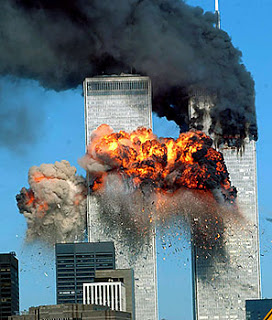
\includegraphics[width=4cm,height=5.5cm]{wtcfire} & 
			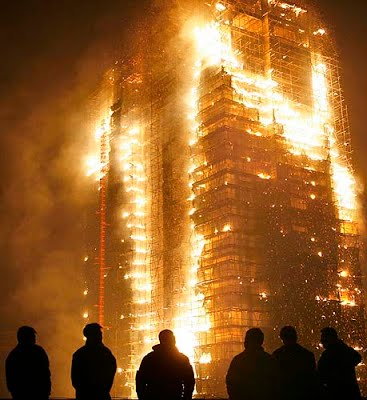
\includegraphics[width=4cm,height=5.5cm]{londonfire} &
			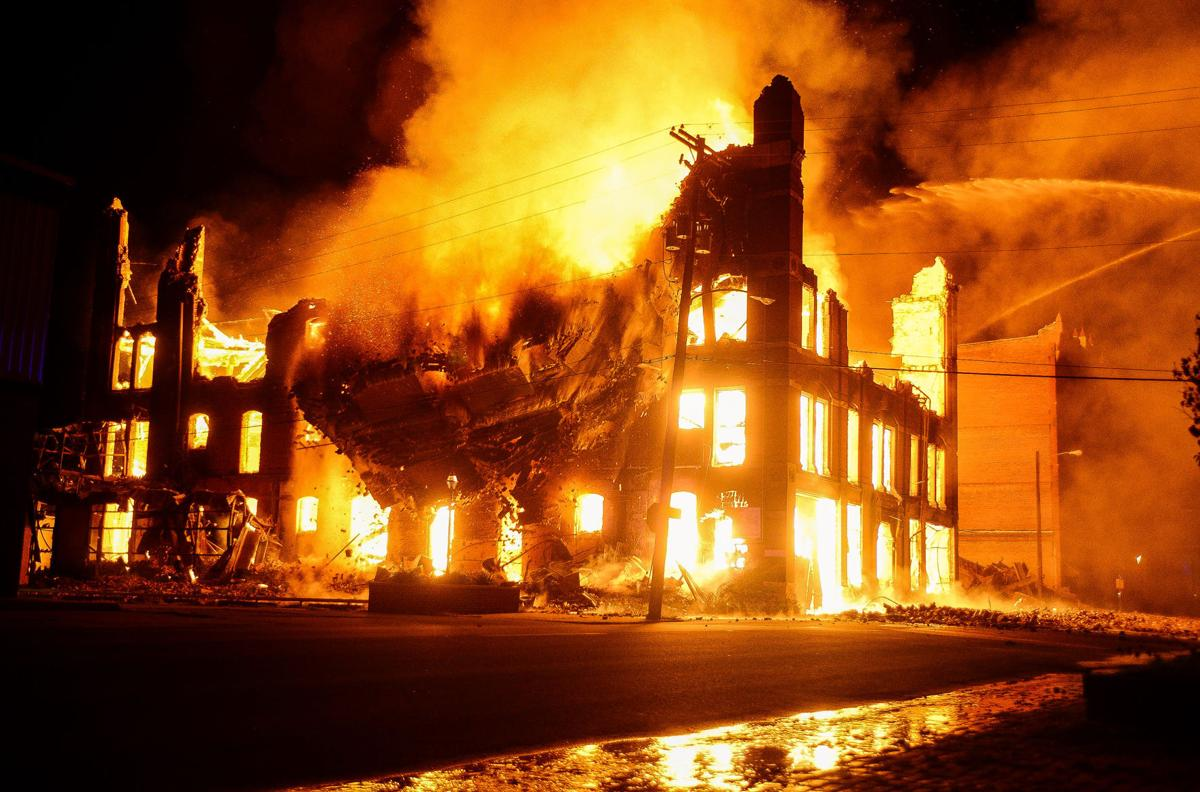
\includegraphics[width=4cm,height=3.5cm]{empirefire} \\ 
			(a) & (b) & (c) \\ 
		\end{tabular} 

	\begin{scriptsize}
	Images extracted from \url{https://images.google.com.au/}
	\end{scriptsize}
	
		\caption{Major fire accidents in recent times}
		\label{fig:Major fire accidents}
\end{figure}

This has led the researchers to concentrate on the fire safety of buildings. Most common form of building constructions include materials which are more susceptible to fire exposure. For instance, the major components of a residential building include concrete, hot-rolled steel and wood. The fire performance of a building is greatly dependent upon the fire performance of these individual materials. Therefore, researchers focus on these materials and are keen to improve the performance of these materials under fire exposure. During a fire incident, the structural elements of a building are subjected to additional fire loads apart from the existing permanent and imposed loads. This results in premature failure of the structural members if they are not properly designed to take the fire loads apart from the structural loads. As this research is focused on the complex LSF walls used in buildings, past literatures with respect to this are summarised.

\section{Experimental and Numerical Investigations of LSF Walls}

The LSF walls used in buildings are load bearing and non-load bearing. The non-load bearing walls are generally used in partition separations in RC framed buildings whereas the load bearing walls are generally found in day to day low rise to mid-rise residential buildings. This section gives a detailed insight of the experimental and numerical investigations carried out on both load bearing and non-load bearing LSF walls in the past.

\citet{Son} experimentally investigated the fire performance of partition walls under load bearing conditions as per ASTM E119-71 standards using two fire tests. The test wall dimensions were 8 foot high and 16 foot long. Lipped channel section of size $3^{\prime\prime}$ $\times$ $1\tfrac{3}{4}^{\prime\prime}$ $\times$ $\tfrac{1}{2}^{\prime\prime}$ inch was used as studs in the former while the latter used tubular sections of $3^{\prime\prime}$ $\times$ $2^{\prime\prime}$ inches as studs in the wall assembly. 18 ga (1.02 mm) thick steel studs were used. Both test walls consisted of two plasterboard sheathed frames separated by $\tfrac{1}{2}^{\prime\prime}$ inch air gap between them. The plasterboards were $\tfrac{5}{8}^{\prime\prime}$ inch inches thick for both fire tests, but the thermomechanical properties of the same are unavailable. Single layer of Type X gypsum plasterboard was used on both test specimens. $3\tfrac{1}{2}^{\prime\prime}$ inch thick glass wool compressed to $3^{\prime\prime}$ inch was used as the insulation. However, the sound insulation values and the material properties were not provided in detail. During the fire tests, the phenomenon of thermal bowing was noticed and reported. Inward thermal bowing was significant, where the test specimen bowed towards the furnace. The first test wall with lipped channel section survived 75 min after which flames were visible on the unexposed side. The second test wall with tubular studs survived 97 min after which visible smoke was seen through cracks on the unexposed side of the test wall. Time-temperature curves were plotted for the plasterboards, but the individual stud time-temperature curves are not available. It was suggested that the usage of two layers of Type X gypsum plasterboard will increase the fire resistance level (FRL).   

The history of fire tests dates back over a century. \citet{Babrauskas1978} summarised the fire tests conducted from 1880 to 1918 and listed the key features in conducting fire tests of walls. Their report was summarised in two parts. The first part reported about the history in forming the fire testing standards, while the second part described the various fire tests carried on different building elements across the globe. It was mentioned that ASTM E119 was the first standard issued on the fire testing of building elements. This report included the major fire tests from the year 1880 and tried to summarise all the fire test reports available in English during that time. However, test reports in other languages were ignored due to the difficulties in interpretation. The need for fire proofing on steel, concrete and timber elements back then was debatable and the necessity for the same was explained. The first report explained in detail about the very first fire test on walls and the difficulties in measuring the temperatures during the fire test. Fire testing of columns were also reported in detail. Details about the fire tests of walls were summarised in the second part of the report.  

It was reported that the first controlled fire test was conducted in Germany in 1891 on a small hut. This emphasised the importance of fire tests over a century ago. The test room was constructed using timber studs and had the dimensions of 2.01 m $\times$ 2.63 m $\times$ 2.63 m. From this report it is evident that until early 1900's the fire tests were conducted on the whole compartment rather than individual building elements. All the fire tests were conducted in a gas-fired chamber, but the dimensions of the test specimens were not consistent. The usage of different organic building elements at different time period were also reported. From the year 1915 it was reported that the furnace dimensions were increased to 3.6 m $\times$ 4.5 m $\times$ 0.4 m. This was the new standard for testing the wall specimens in Underwriters Laboratory (UL) and thermocouples were used for temperature measurements instead of thermometers. Apart from the tests on walls, the report also elaborated the fire tests of other building components such as doors and openings. However, temperature distribution across the wall was not reported in detail. The establishment of the standard fire curve in the year 1917 and the inclusion of the same into the ASTM E119 standards was also described in detail. This also included various failure criteria for different building elements and their level of fire protection. Also, the validation checks conducted to verify the suitability of the standard fire curve was also discussed in detail.

\citet{Klippstein1978} used the fire test results conducted on LSF walls based on ASTM E119 to propose analytical methods to predict the structural failure time of gypsum plasterboard sheathed LSF walls. Initially, he conducted tests to determine the mechanical properties of the steel sections used in the LSF walls. The test walls used for this study were 3.05 m $\times$ 3.05 m. Only the axial loads were considered in the fire design while the wind loads were neglected in the calculations. The phenomenon of plasterboards not providing effective lateral restraints to the studs at elevated temperatures was discussed in detail. The concept of unequal load sharing in LSF walls was also discussed, i.e., higher load carried by the stronger studs (less temperatures) during full-scale fire test. Failure of the stud was assumed to happen by weaker axis buckling in formulating the design equations. The concept of load ratio (LR), $P_T/P$, was used, where $P_T$ is the calculated failure load at elevated temperature $T$ while P is the failure load at ambient temperature. The failure load was determined theoretically using the following equation.
\begin{equation}
	P = \dfrac{23}{12} F_{al}A
\end{equation}
Elastic buckling was the governing failure mode in studs more than 4.5 m height assuming pinned end conditions. As the studs in LSF walls are generally 3 m tall, inelastic buckling was the critical failure mode. The equation to predict the inelastic buckling load was proposed as shown next. 
\begin{equation}\label{eq:inelastic}
	F_{al} = \dfrac{12}{23} QF_y-\dfrac{3}{23}\dfrac{(QF_y)^2}{\pi^2E}\left(\dfrac{KL}{r}\right)^2 	
\end{equation}
Where
\begin{description}[itemsep=0pt,parsep=0pt]
	\item $Q$ = strength reduction factor at room temperature
	\item $F_y$ = actual yield strength at room temperature
	\item $E$ = modulus of elasticity at room temperature
	\item $K$ = effective length factor of the stud
	\item $L$ = length of the stud
	\item $r$ = radius of gyration about the major axis.
\end{description}	
Based on the above \Cref{eq:inelastic} the failure load at room temperature was determined using the next equation.
\begin{equation}
	P = \left[QF_y - \dfrac{1}{E}(\dfrac{QF_yL}{2\pi r})^2\right]A
\end{equation}
During the fire test, the studs deflect laterally causing bending stresses and these effects have to be included in calculating \(P_T\). Therefore, the interaction equation for combined axial and bending action available in the AISI manual was used and is shown next.
\begin{equation}
	\dfrac{f_a}{F_{alT}} + \dfrac{C_{mx}}{\left(1-\dfrac{f_a}{F'_e}\dfrac{f_b}{F_{blT}}\right)} < 1.0
\end{equation} 
Where
\begin{description}[itemsep=0pt,parsep=0pt]
	\item $f_a$ = compressive stress due to axial load
	\item $F_{alT}$ = allowable stress for axial load at failure temperature
	\item $\dfrac{C_{mx}}{\left(1-\dfrac{f_a}{F'_e}\dfrac{f_b}{F_{blT}}\right)}$ = modification factor for bending stresses
	\item $f_b$ = bending stress at mid-height
	\item $F_{blT}$ = allowable bending stress at failure temperature
	\item $F_{yT}$ = allowable strength at failure temperature
	\item $Q_T$ = column-strength reduction factor at failure temperature
	\item $E_T$ = modulus of elasticity at failure temperature
\end{description}
Based on the above mentioned equations the load ratio (LR) was computed by the following equation.
\begin{equation}
	LR = \dfrac{1}{\left(\dfrac{1}{F_{alT}}+\dfrac{23 A \delta _T}{128_xF_{yT}}\right)F_{al}}
\end{equation}
To determine the capacity reduction in the members, elevated temperature material properties were determined and used in the above mentioned equations. It was found that at elevated temperatures, the elastic modulus of sheet steel decreased rapidly in comparison with that of plate steel. Stub column tests were also conducted to determine the column strength reduction factors at elevated temperatures. The proposed equations resulted in conservative results in comparison with the experiments.

\citet{Gerlich1996} investigated the design of LSF walls under standard ISO 834 fire curve and some real fire curves. They proposed suitable methods for calculating the reduction in strength ofLSF wall at elevated temperatures, and the stud deflections caused by elevated temperature gradients and P-$\Delta$ effects. Three design standards, AS 1538, BS 5950 and AISI specifications were compared for the limit state design of cold-formed steel sections at room temperature. It was found that the AISI design manual gave accurate capacity predictions. The experimental structural test was initially conducted for 3m length columns under axial loads and bending to verify the AISI design method at ambient conditions. An equation for specific heat (k) until 900\degree C of fire exposure was also developed.

\begin{equation}
k = -0.022T + 48, for 0 < T < 900\degree C
\end{equation}

It was concluded that with the help of experimental and analytical studies, the P-$\Delta$ effect at elevated temperatures can be predicted with good accuracy. Buckling of the compression flange of cold-formed steel stud on the ambient side was the main cause of structural failure at elevated temperatures.

\citet{Alfawakhiri1999} reviewed the fire resistance of load bearing steel stud walls protected with gypsum board. They suggested that there were robust experimental methods to test the thermal performance of LSF walls, but there was a gap in the numerical analyses and the design procedures for LSF walls. The importance of using insulation such as mineral wool, glass fibre, cavity insulation etc, within the wall was highlighted. The thermal conductivity of various gypsum boards was discussed and a relationship was established between thermal conductivity and temperature. Likewise, the relationship between specific heat and temperature was also developed. The variation in the modulation of elasticity of the cold-formed steel sections with respect to temperature was also reviewed. It was concluded that factors such as specific heat, thermal conductivity and modulus of elasticity of studs with variation in temperature will have a significant effect on the fire performance of steel studs.   

\citet{Sultan2000a} summarised the performance based parameters to be considered in designing LSF walls in fire. Seventeen full-scale fire tests conducted previously were considered as reference for this study. All the considered wall specimens were 3 m high and 3.7 m wide. Both steel and wood stud assemblies were considered in this study. However, the wall specimens were lined using gypsum plasterboard only. All the steel stud assemblies considered were non-load bearing. The reference fire tests were conducted in accordance with CAN/ULC-S101-M89 (\citeyear{ULC1989}). It was found that the presence of cavity insulation resulted in rapid increase of the plasterboard temperatures in comparison with uninsulated wall assemblies. The average temperature on the unexposed side of the test wall was lower in specimens with rock fibre insulation in comparison with non-insulated assemblies. The use of cavity insulation in non-load bearing LSF wall assemblies resulted in increased FRL. However, the effects of insulation in loadbearing LSF walls were not discussed in detail. It was also reported that, the type of insulation did not significantly affect the FRL, provided the insulation had a perfect fit between the studs resulting in no loose gaps.

Another important finding was that the presence of resilient channels and proper positioning of the same, significantly increased the FRL in non-load bearing LSF wall assemblies. However, the effective restraints provided by the resilient channels along with the plasterboards were not reported in detail, as all the LSF wall tests were conducted under non-load bearing conditions. The presence of second layer of plasterboard with staggered joint arrangement significantly increased the FRL in comparison with single plasterboard layer. It was reported that under non-load bearing conditions, the type of stud such as wood or steel did not affect the FRL.  

\citet{Collier2002} reviewed the BRANZ method of height extrapolation to study the resistance of non-load bearing steel framed walls under fire. The wall specimen chosen was set at 4 m $\times$ 4 m panel in comparison to the conventional 3 m $\times$ 3 m panel. The horizontal joints appeared to fail prematurely in comparison with vertical joints when exposed to fire. This premature failure can expose the stud flanges directly to fire. This research also compared the test results of wall panels with and without vertical lining joints.

\citet{Feng2003c} studied the thermal performance of cold-formed thin-walled steel panel systems in fire using small-scale fire tests of 1.5 $\times$ 1.5 $\times$ 1.5 m wall panels made of lipped channel studs with and without service holes. The performance of gypsum board in fire was the principal focus of this research. Focus was given in developing a finite element model to predict the thermal performance of gypsum boards and steel studs. Time-temperature curves were plotted for panels tested with different layers of gypsum board and insulation under fire. ABAQUS finite element analyses (FEA) were conducted using the material properties of gypsum board, steel studs and insulation in BS EN 1993-1-3 (2006) Part 1.2. Tests and FEA results and several conclusions were made as follows. The free water content present in the gypsum boards was not considered in the numerical analysis. Hence the results from FEA were reasonable, but were not accurate in accordance with the experimental results. Different layers of gypsum boards along with insulation on the fire side were used both in experiments and analyses and it was found that the steel stud temperature had a high influence on the usage of insulation and not the number of layers of gypsum board on the exposed side. It was concluded that increasing the number of gypsum boards increased the FRL. The failure of gypsum boards on the exposed face, did not promote fire spread to the unexposed face due to the presence of insulation. Isowool and Rockwool insulations were used and the results were compared with a non-insulated wall panel. It was found that, the presence of insulation on the fire exposed side of the wall resulted in higher stud temperature. The thermal performance of the wall might get affected if the insulation is provided on the unexposed face of the wall to reduce cold bridging in warm construction. The shape of the thin-walled cold-formed steel cross section had the least effect on the thermal performance, whereas in the case of a cassette section the thermal performance was affected by its layout.  

Based on the fire test results \citet{Feng2003d} then investigated the structural behaviour of LSF wall panels. Numerical analysis and design calculation were carried out based on 52 channel sections with FE package ABAQUS. Modified design equations for channel sections were proposed to include the effects of distortional buckling failure and change in strength and stiffness of steel at elevated temperatures based on BS5950 Part 5 and Eurocode 3 Part 1.3. They also included the service holes present in the steel studs, and their effect on the ultimate strength based on AISI (1996). The geometric non-linearities, imperfections and stress-strain relationships at elevated temperatures based on Eurocode 3 Part 1.2 or \citet{Outinen1997} were also considered. The equation for calculating the effective width of a flange for distortional buckling was modified as follows.

\begin{equation}
\dfrac{b_{eff,de}}{b}= 1~for~\lambda \leq 0.673
\end{equation}
\begin{equation}
\dfrac{b_{eff,de}}{b}= \sqrt{\dfrac{\sigma_{de}}{f_y}}\bigg(1-0.22\sqrt{\dfrac{\sigma_{de}}{f_y}}\bigg)~for~\lambda \geq 0.673
\end{equation}

Based on the design modifications and numerical analysis, it was concluded that the design formulations used for ambient capacity calculation can be extended and used for elevated temperatures as well. This is achieved, when the reduced yield strength derived from 0.2\% proof stress and the reduced elastic modulus are used. The effect of distortional buckling can be included in the design calculations based on \citet{Young1992}. Service holes can be considered in the design, based on AISI specifications. ABAQUS FE models can be used to stimulate the behaviour of cold-formed steel sections at elevated temperatures, provided proper material properties and boundary conditions are used. \citet{Feng2003} extended the study to investigate the axial strength of CFS channels under non-uniform elevated temperatures due to fire. Two methods were adopted for the design process. First the EN1993-1-3 ambient temperature design equation was modified and the second using the limiting temperature method. The design equations for the cold-formed steel columns under combined axial load and bending moments were based on the following equations from Eurocode 3 Part 1.2.

\begin{equation}
\dfrac{N_{sd}}{\chi_{min}f_{yb}A_{eff}}+\dfrac{k_y(M_{y,sd}+\Delta M_{y,sd})}{f_{yb}W_{eff,y,com}}+\dfrac{k_y(M_{z,sd}+\Delta M_{z,sd})}{f_{yb}W_{eff,z,com}} \leq 1
\end{equation}

\begin{equation}
\dfrac{N_{sd}}{\chi_{lat}f_{yb}A_{eff}}+\dfrac{k_y(M_{y,sd}+\Delta M_{y,sd})}{f_{yb}W_{eff,y,com}}+\dfrac{k_y(M_{z,sd}+\Delta M_{z,sd})}{f_{yb}W_{eff,z,com}} \leq 1
\end{equation}

Later the results from the modified design equations from the EN1993-1-3 were compared with ABAQUS simulation results based on S4R shell FE models. 100 x 54 x 15 x 1.2 mm lipped channel sections were used in the study. Appropriate restraints were applied to the studs to simulate the full-scale fire test conditions. Sequential uncoupled FE analysis was conducted and the results showed that failure temperatures of the stud sections were similar in the experimental and numerical studies irrespective of the number of plasterboard layers. The use of more than one layer of plasterboard delayed the temperature of the studs. 

\citet{Sakumoto2003} conducted ISO 834 standard fire tests of walls and floors using various light gauge steel stud shapes. Partition walls and exterior walls were the main aim of the study. The wall specimens of 1820 $\times$2700 mm consisted of 0.5 to 1.6 mm studs and 12.5 mm thick plasterboards. Unlike other fire tests, the partition walls consisted of two rows of studs separated by 9 mm plywood. The studs were lipped channel sections with different depths ranging from 89 mm to 235 mm and were spaced at 500 mm centres. Two layers of non-fire rated plasterboards were present on either side of the wall and an axial load of 34 kN was applied to some specimens. Glass wool insulation was present in both cavities of the partition wall, which resulted in the highest FRL. The fire tests for the partition walls were carried out by varying the studs and the configuration with plywood between the rows of stud resulted in the highest with 67 min of FRL. Likewise different floor-ceiling configurations of 2950 mm$\times$ 4260 mm were also tested. It was concluded that the gypsum board fall-off was an important criterion in determining the FRL. The plasterboard fall-off can be reduced by increasing the number of plasterboard layers. The collapse temperature, time and sequence of failure of the structural members in the LSF wall were also detailed. Most of the tests conducted on wall panels had single layer plasterboards and the FRL was about 45 min. In the case of wall panels with plywood the FRL was just above 60 min. 

\citet{Feng2005} investigated the cold-formed, thin-walled steel panels with service holes in fire. The holes were provided in the channel sections, one near the top and one near the bottom. Full-scale tests were carried out at different load ratios of 0.2, 0.4 and 0.7. The main observation in the failure of the steel studs was that the studs failed by local buckling near the service holes at ambient temperature. Flexural-torsional buckling along the major axis with lateral deflection caused by thermal bowing due to the temperature gradients was also observed. Increase in the stud temperature was noticed during some tests due to the complete burning of the insulation layer. Detachments of the fasteners along the unexposed side of the panels were also noticed during the test. 

\citet{Manzello2005} studied the performance of partition assemblies under real fire conditions. This research was different from others as their fire test was performed in real-scale compartment instead of a conventional furnace setup. This test was carried out for non-load bearing conditions. A compartment shown in \Cref{fig:manzello_compartment} was constructed, the fire curve based on ASTM E119 was simulated within the compartment and the thermal performance of the partition walls was investigated. Thermocouples, infra-red cameras, normal cameras and heat flux sensors were used for the test. It was observed that the rate of temperature rise on the plasterboard surfaces was higher compared to those tested in the furnace. It was also reported that the total heat flux measured was dependent on the wall height. But the rate of increase of the heat flux was smaller when compared to the furnace fire test. Numerical simulations the experiments were then performed by \citet{Manzello2007}. The model was entirely mathematical instead of widely used FE models. It was able to predict the fire behaviour only upto certain level of precision due to the effects of smoke movement, plasterboard fall-off etc.
\begin{figure}[htbp]
	\centering
		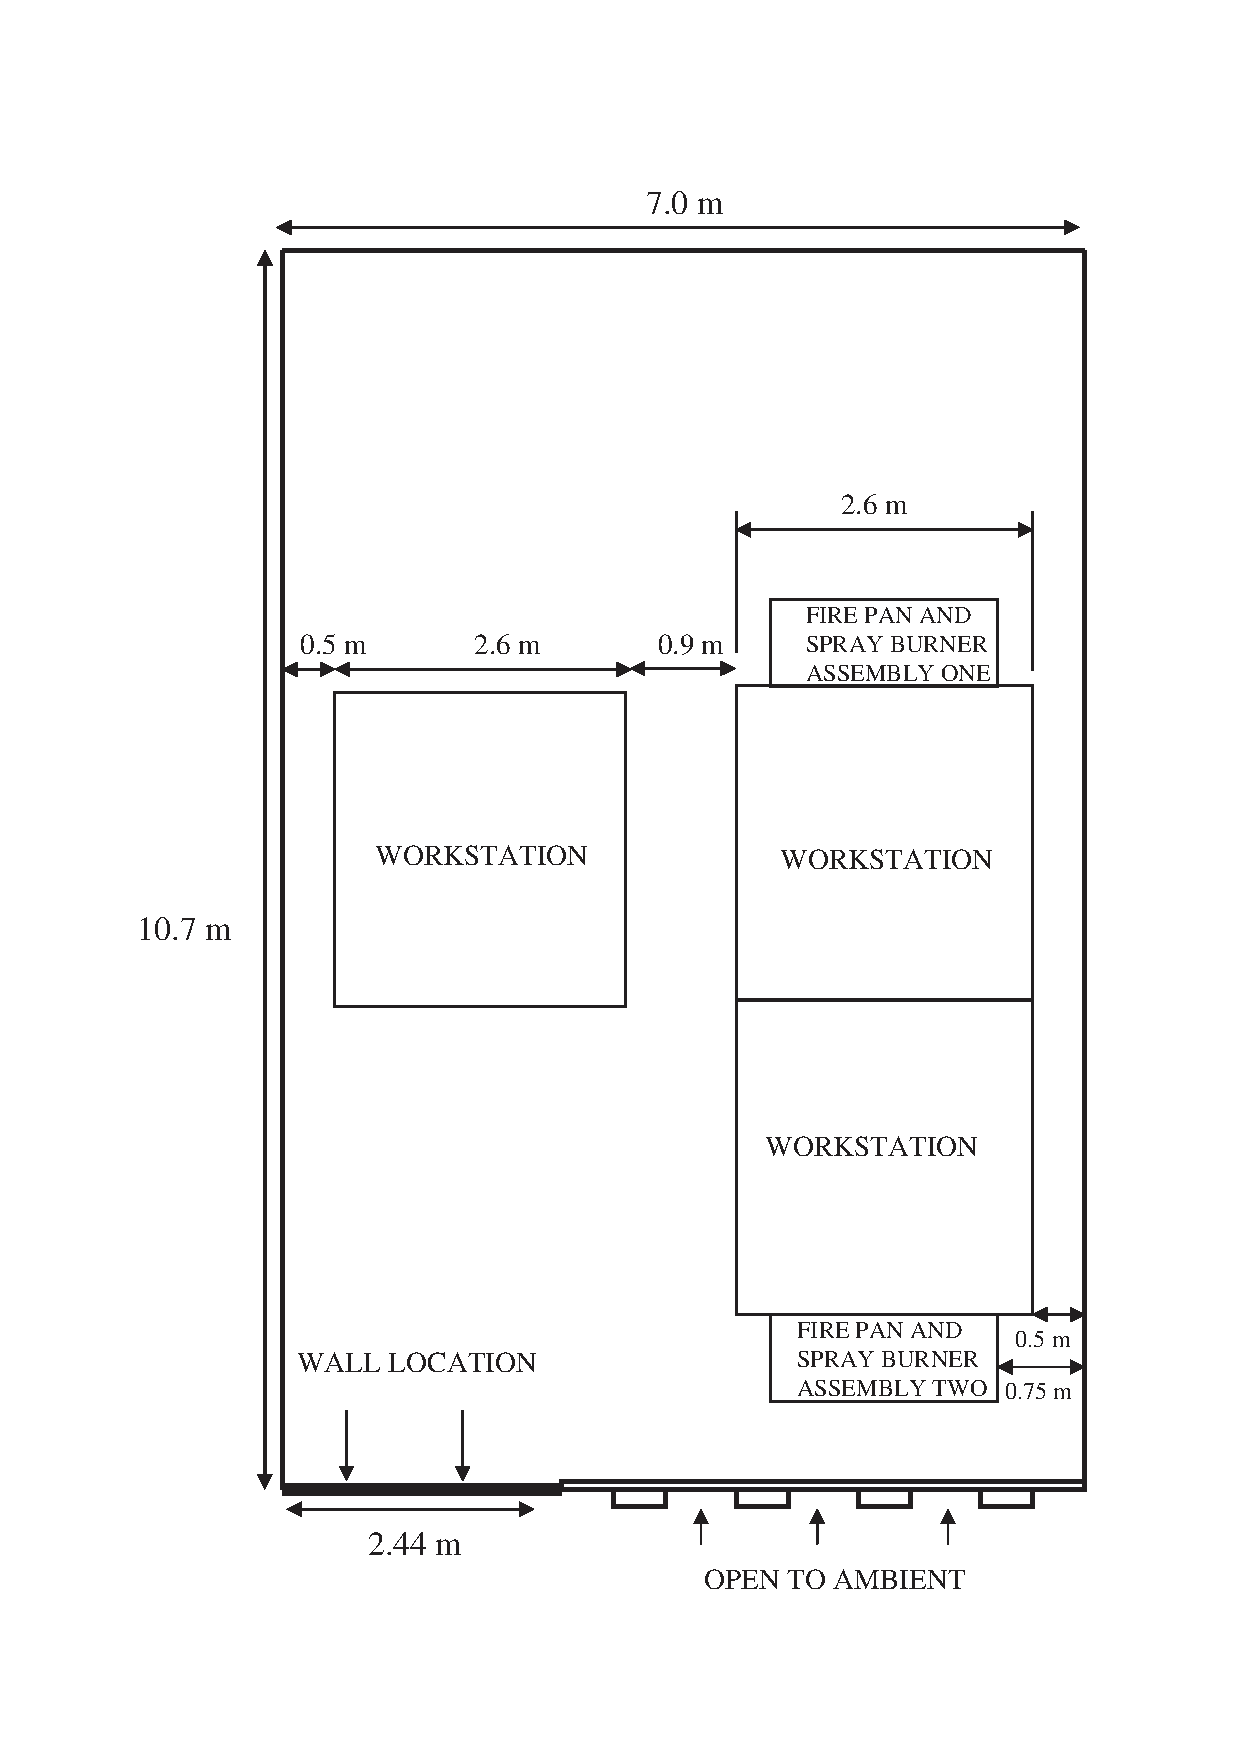
\includegraphics[width=6cm,height=10cm]{manzello_compartment}		
		\caption{Compartment dimensions used by \citet{Manzello2005}}
			\label{fig:manzello_compartment}
	\end{figure}

\citet{Kodur2006} investigated the important factors that influenced the fire resistance of load bearing steel stud walls. Spacing of the studs and their thickness of the steel used, the magnitude of load acting on the panel, shear membrane and type of installation were the parameters analysed by them. It was found that the insulation type and the number of layers of gypsum board in the panel were highly influential, The use of cavity insulation was shown to reduce the fire rating of the wall assemblies. Increasing the layers of plasterboard resulted in higher fire resistance. Provision of the OSB shear membrane in place of gypsum boards in load bearing wall panels resulted in the deterioration of fire resistance. Studs arranged in a staggered manner in two rows resulted in higher fire resistance when compared to a single layered stud arrangement. It was discussed that this higher fire resistance of the double layered staggered stud arrangement was due to the larger heat sink caused by the larger cavity within the wall. Another finding was that MSG 20 light steel section performed better than ordinary MSG 20 section in providing fire resistance.

\citet{Knobloch2006} proposed a strain based approach to local buckling of steel sections exposed to fire. Generally, stress based design approach based on ambient temperatures is used to design them. Unaltered effective width and a reduced 0.2\% proof stress based yield strength were only used for elevated temperature design. This has resulted in unsatisfactory design results. Hence, a strain based method was developed for unstiffened and stiffened elements of CFS members. Strength curve based on yield line theory considering the initial imperfection was also formulated. Calculations are done based on the proposed design methods and compared with the results from the numerical analysis. The procedure involved in this proposed design is as follows. 
\begin{itemize}
	\item For different support conditions the non-dimensional slenderness at elevated temperature is determined.
	\item Then the reduction factor for plate buckling at elevated temperature \(\rho\theta\) is calculated based on \citet{Desmond1981},  also known as Winter’s equation as shown next.
	\begin{equation}
	\rho \theta = \dfrac{1}{\bar{\lambda}_{\rho \theta}}\Bigg(\dfrac{1-0.22}{\bar{\lambda}_{\rho \theta}}\Bigg) 
	\end{equation}
	\item Later the effective width is calculated using the proposed stress-strain relationships at elevated temperatures and the stress distribution of the element is obtained.
	\item Finally, the axial and bending moment resistances are calculated by integration.
\end{itemize}
\begin{figure}[htbp]
	\centering
		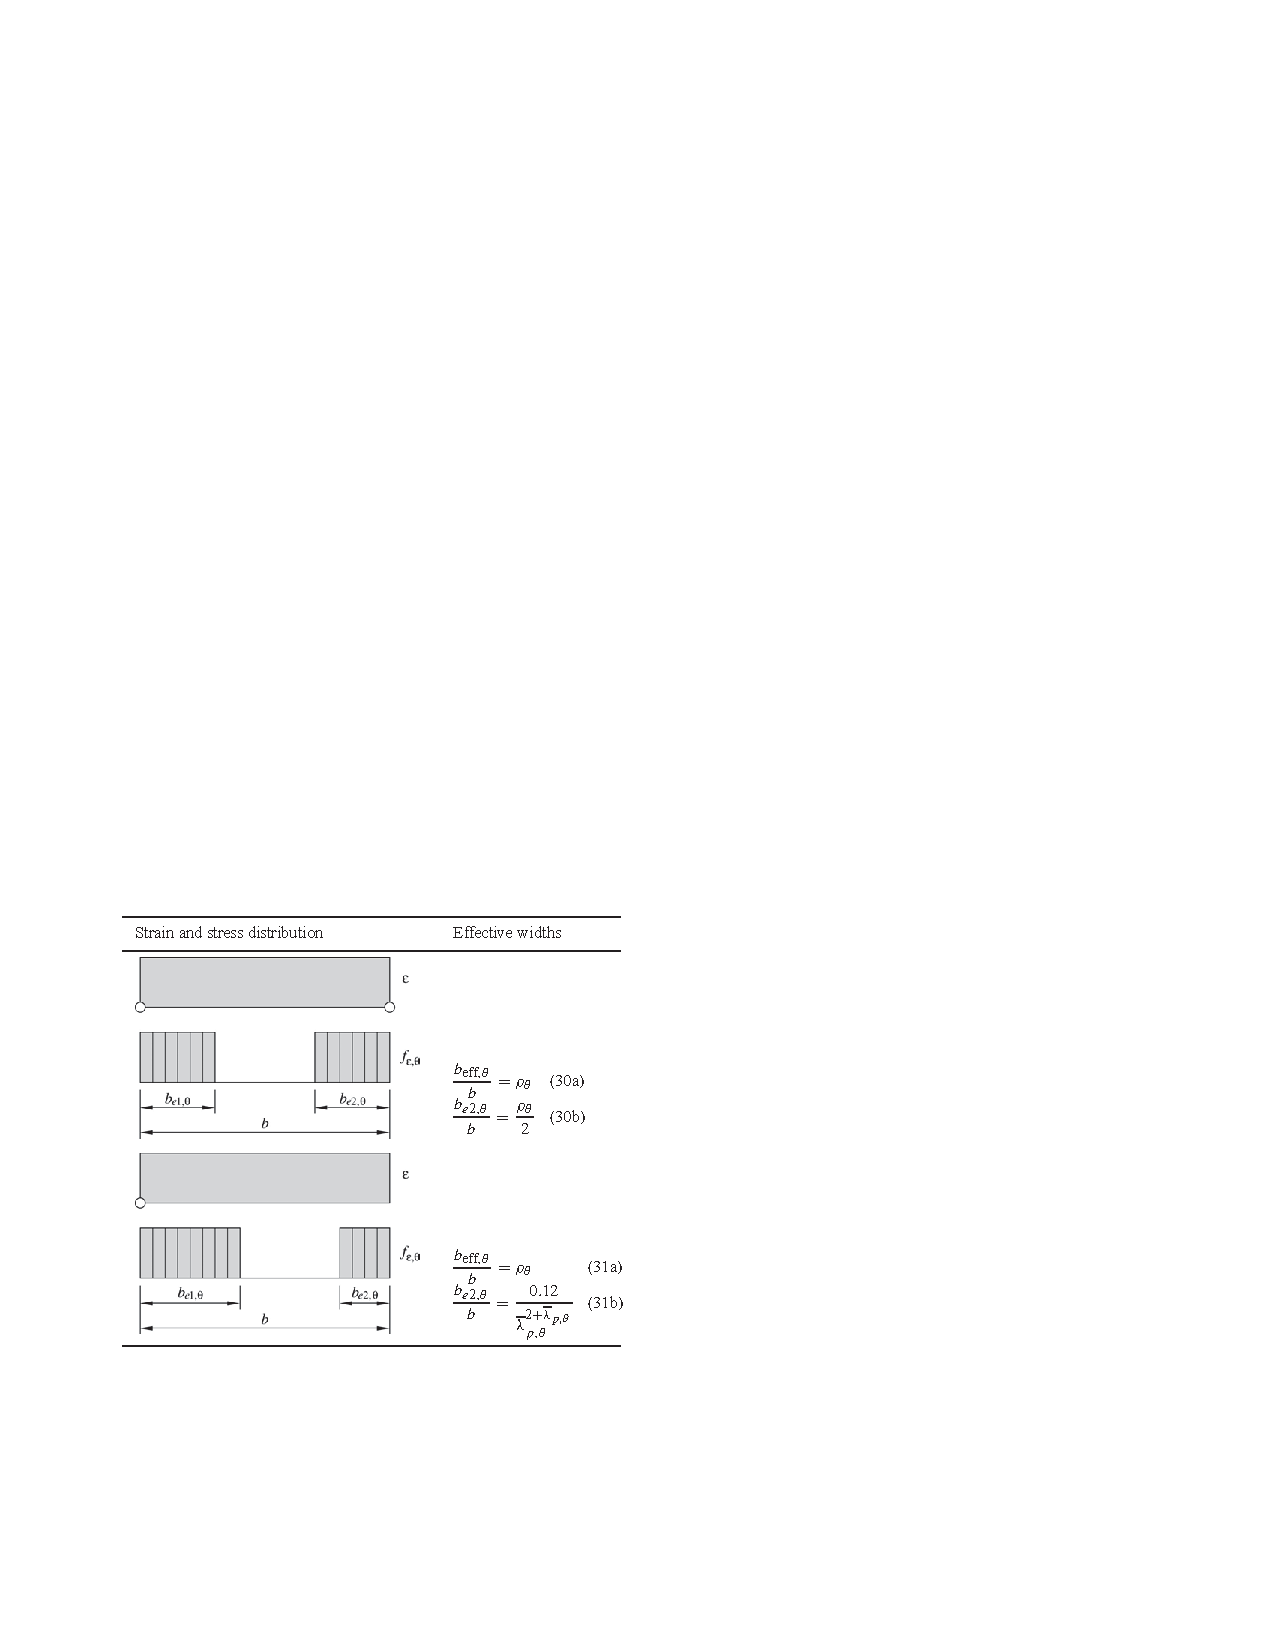
\includegraphics[width=10cm,height=10cm]{knobloch_effwidth}		
		\caption{Proposed effective width table from \citet{Knobloch2006}}
			\label{fig:knobloch_effwidth}

	\end{figure}

The proposed effective width formulae for unstiffened and stiffened elements are as shown in \Cref{fig:knobloch_effwidth}. The proposed effective width formula for unstiffened and stiffened elements are as shown in \Cref{fig:knobloch_effwidth}.It was concluded that, the local buckling of the studs and the additional capacity due to the plastic behaviour of cross section had a strong influence on the resistance the steel in fire. Also, the local buckling was dependent largely on strain. 

Experimental investigation of different cold-formed steel materials at elevated temperatures were conducted by \citet{Chen2007}. Primary focus of this research was to report the material properties of cold-formed steels at elevated temperatures. Elevated temperatures tensile coupon tests at elevated temperatures of G550 and G450 grade steels with varying thicknesses were conducted to determine the elastic modulus and yield strength at different strain levels, ultimate strength, ultimate strain and thermal elongation for comparison with Australian, British and Eurocode Standards. A unified equation to predict the above mentioned material properties was also proposed. Comparisons between the test results and proposed equations were also carried out. Both transient and steady state methods were used in the tensile coupon tests. But the transient method is more practical in real time fire exposure. Yield strengths at 0.5\%, 1.5\% and 2\% strain levels were obtained and comparisons among them were undertaken. Serration was observed on the stress-strain curve at high temperatures. Static drop was obtained in the stress-strain curve at room temperature of 22\degree C. This was achieved by pausing the strain applied for 1 minute thereby allowing the stress relaxation associated with plastic strain. This reduces the effect of loading rate. A series of tests was also conducted to study the effects of static drop at different temperatures. Based on the experimental investigations, an equation for determining yield strength, ultimate strength and ultimate strain of cold-formed steels was proposed as follows.

\begin{equation}
\text{Yield Strength} \to \dfrac{f_{0.2,T}}{f_{0.2,normal}} = a-\dfrac{(T-b)^{n}}{c}
\end{equation}

\begin{equation}
\text{Ultimate Strength} \to \dfrac{f_{u,T}}{f_{u,normal}} = a-\dfrac{(T-b)^{n}}{c}
\end{equation}

\begin{equation}
\text{Ultimate Strain} \to \dfrac{\epsilon_{u,T}}{\epsilon_{u,normal}} = a-\dfrac{(T-b)^{n}}{c}
\end{equation}

A modified stress-strain curve model based on the Ramberg-Osgood model was proposed as follows.

\begin{equation}
\epsilon_T = \dfrac{f_T}{E_T}+0.002\big(\dfrac{f_T}{f_{y,T}}\big)^{nT} for f_T \leq f_{y,T}
\end{equation}

\begin{equation}
\epsilon_T = \dfrac{f_T-f_{y,T}}{E_{y,T}}+\epsilon_{u,T}\big(\dfrac{f_T-f{y,T}}{f_{u,T}-f_{y,T}}\big)^{mT} + \epsilon_{y,T} for f_T > f_{y,T}
\end{equation}

Where

\begin{equation}
E_{y,T} = \dfrac{E_T}{1+0.002n_TE_{y,T}/f_{y,T}}
\end{equation}

\begin{equation}
n_T = 20-0.6\sqrt{T}
\end{equation}

\begin{equation}
m_T = 1+\dfrac{T}{350}
\end{equation}


From this study, it was concluded that the Australian, British and European standards were conservative in predicting the yield strength, elastic modulus and thermal expansion except for G550 1 mm steel between 450\degree C to 970\degree C and for G450 1.9 mm steel at 600\degree C. 

\citet{Kolarkar2008} studied the thermal performance of LSF walls with double layer plasterboards, where the insulation was sandwiched between the plasterboards externally. The investigation was conducted by using small-scale fire tests of non-load bearing LSF walls exposed to the standard fire curve. It was found that sandwiching of insulation externally between the plasterboards resulted in better thermal performance when compared to traditional stud walls with cavity insulation. 

\citet{Ranawaka2009} investigated the distortional buckling behaviour of cold-formed steel compression members at elevated temperatures. Lipped and Unlipped channel compression members were tested at temperatures ranging from 20 to 800\degree C. Their ultimate compression capacities from the tests were compared with design code predictions. The distortional ambient temperature buckling capacities from the tests were compared with those predicted by direct strength and buckling strength equations in AS/NZS 4600 and were found to agree well. At elevated temperatures, the reduced mechanical properties were used to predict the compression capacities, in which case the comparison with the test results showed that the AS/NZS 4600 design equations were over-conservative.

\citet{Rahmanian2011} conducted 12 medium-scale (1 m $\times$ 1 m) standard fire tests of LSF walls under load bearing conditions. The number of plasterboard layers was varied to study the thermal behaviour of gypsum plasterboard assemblies using different types of plasterboards. The concept of cyclic condensation-evaporation of the moisture content in the plasterboard during fire tests was also investigated. Material property tests were also conducted on various gypsum plasterboards to study the effect of moisture transfer in gypsum plasterboard assemblies and the data was used to develop thermal finite element models in ABAQUS. 

\citet{Chen2012a} conducted five full scale fire tests of conventional single stud load bearing LSF wall systems lined with different types of fire protective boards including gypsum plasterboard. Bolivian magnesium boards and calcium silicate boards were used in this study. Load ratios of 20\%, 40\% and 70\% were used in the fire tests. Fire tests showed that the load bearing LSF walls without cavity insulation provided better FRL when compared to those with cavity insulation. Also, the thickness of the stud section influenced the FRL. Thicker the stud higher was the FRL. This effect was reported by previous researchers also. It was concluded that the calcium silicate boards when used as the base layer provided better fire performance than gypsum plasterboards. However, due to the spalling behaviour of calcium silicate boards at higher temperatures, it does not possess a noticeable advantage than compared to gypsum plasterboards. Bolivian magnesium oxide plasterboards performed better in fire when compared to gypsum plasterboards. Staggered arrangement of boards were followed in the fire tests, but there were no significant changes in the steel temperatures when compared with conventional plasterboard arrangement. 

\citet{Kolarkar2012} investigated the fire performance of LSF walls using small-scale fire tests. Nine small-scale tests were conducted under to ISO 834 standard time-temperature exposure. A novel LSF wall configuration of external insulation was introduced and its fire performance was investigated using small-scale fire tests. The test wall dimensions were 1280 mm $\times$ 1015 mm. Insulation materials such as glass fibre, rock wool and cellulose were considered. The following findings were drawn from this research.
\begin{itemize}
	\item Presence of plasterboard joints did not significantly affect the thermal performance, in comparison with the tests without plasterboard joints in small-scale fire test. However, the plasterboard joints can have a significant effect during full-scale fire tests and under load bearing conditions.
	\item LSF test walls with single plasterboard configurations tend to exhibit steep rise in temperatures as the plasterboard calcinates after 20 min of fire test. This leads to premature structural failures in load bearing LSF walls when exposed to fire.
	\item Heat transfer in non-cavity insulated LSF walls was more uniform in comparison with cavity insulated LSF walls resulting in reduced thermal bowing of the LSF wall.
	\item The studs of LSF walls with rock fibre insulation resulted in higher temperatures on the hot flanges while the stud temperatures of LSF walls with cellulose insulation were the lowest. This indicates that the non-uniformity in temperature distribution is the highest in LSF walls with rock fibre insulation and can result in premature structural failures under load-bearing conditions.
\end{itemize}

\citet{Gunalan2013e} investigated experimentally the behaviour of 11 full-scale (2.4 m $\times$ 2.4 m) load bearing LSF wall systems exposed to ISO fire curve (\Cref{tab:gunalan_experiments}). This research focused on the LSF walls used in Australia. Conventional LSF wall assemblies with single row of studs were used in this research. The LSF wall panel arrangement was made of four studs connected by tracks on top and bottom. Noggings were not used in any of the wall panels. The wall panels had different kinds of insulation such as glass fibre, rock fibre and cellulose fibre. New LSF panels by sandwiching insulation between the plasterboards (external insulation) were also developed as part of this research. The studs used were 92 $\times$ 40 $\times$ 15 $\times$ 1.15 (G500) lipped channel sections with varying number of plasterboard layers (one or two). Load ratios of 0.2 and 0.4 were used (9 and 2 tests). It was found that providing external insulation in the load bearing LSF walls significantly improved the FRL of the wall system even at higher loads. 
\begin{table}
	\centering
	\caption{Test wall configurations used by \citet{Gunalan2013e}}
		\begin{tabular}{c}
			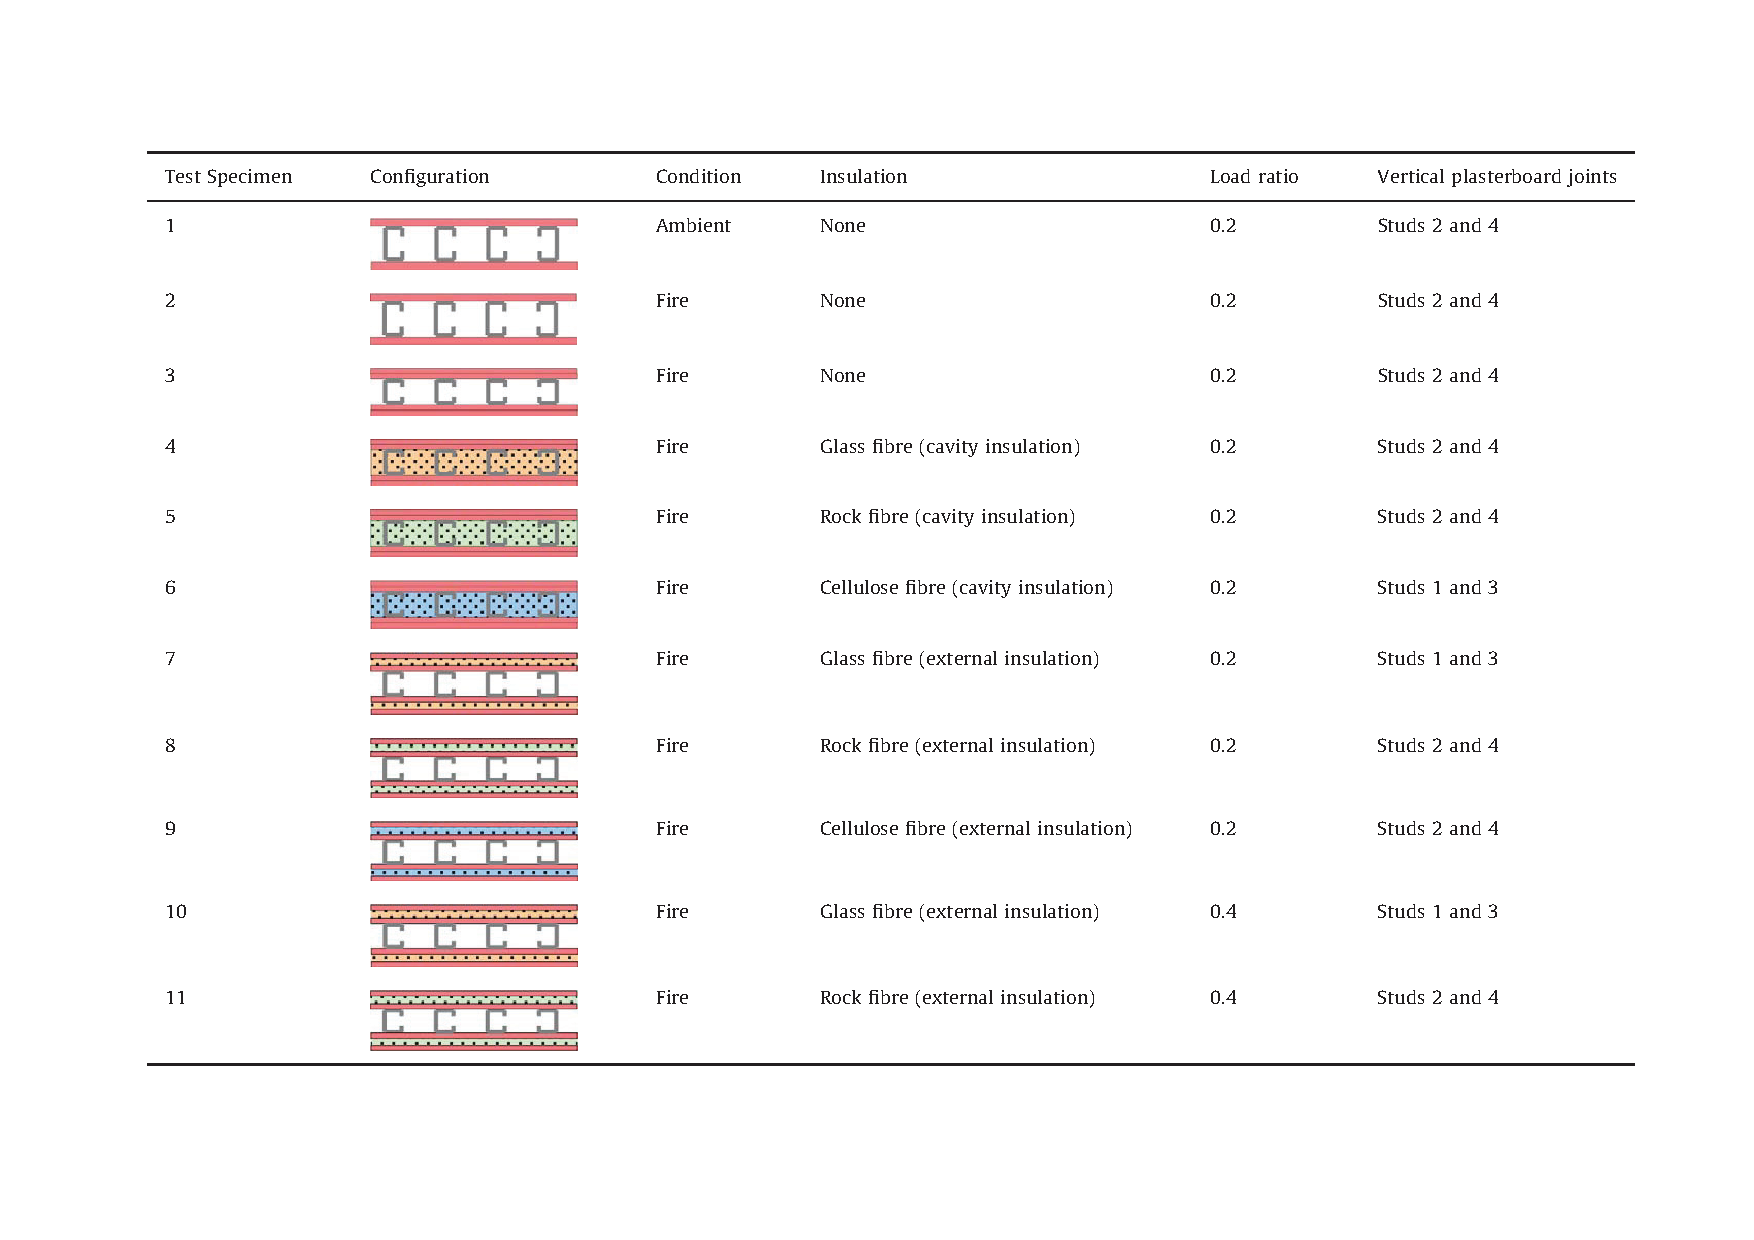
\includegraphics[width=14cm,height=10cm]{gunalan_experiments}	
			\label{tab:gunalan_experiments}
		\end{tabular}
\end{table}

\citet{Chen2013} investigated different types of plasterboard and insulation materials to improve the fire performance of load-bearing LSF wall systems. Plasterboard types such as gypsum plasterboard, oriented standard boards (OSB), Bolivian magnesium board, rockwool boards and autoclaved lightweight concrete (ALC) boards were used in this research. Aluminium silicate insulation was also used in the full-scale fire tests. Total of six full-scale fire tests were conducted for this research. The experimental setup included lipped channel stud sections with depth varying from 89 to 140 mm. Back to back lipped channel stud sections were used in the fire tests with higher load ratios. \Cref{fig:chen2013_test} shows the typical failure of studs in the test wall after the fire test. 
\begin{figure}[htbp]
	\centering
		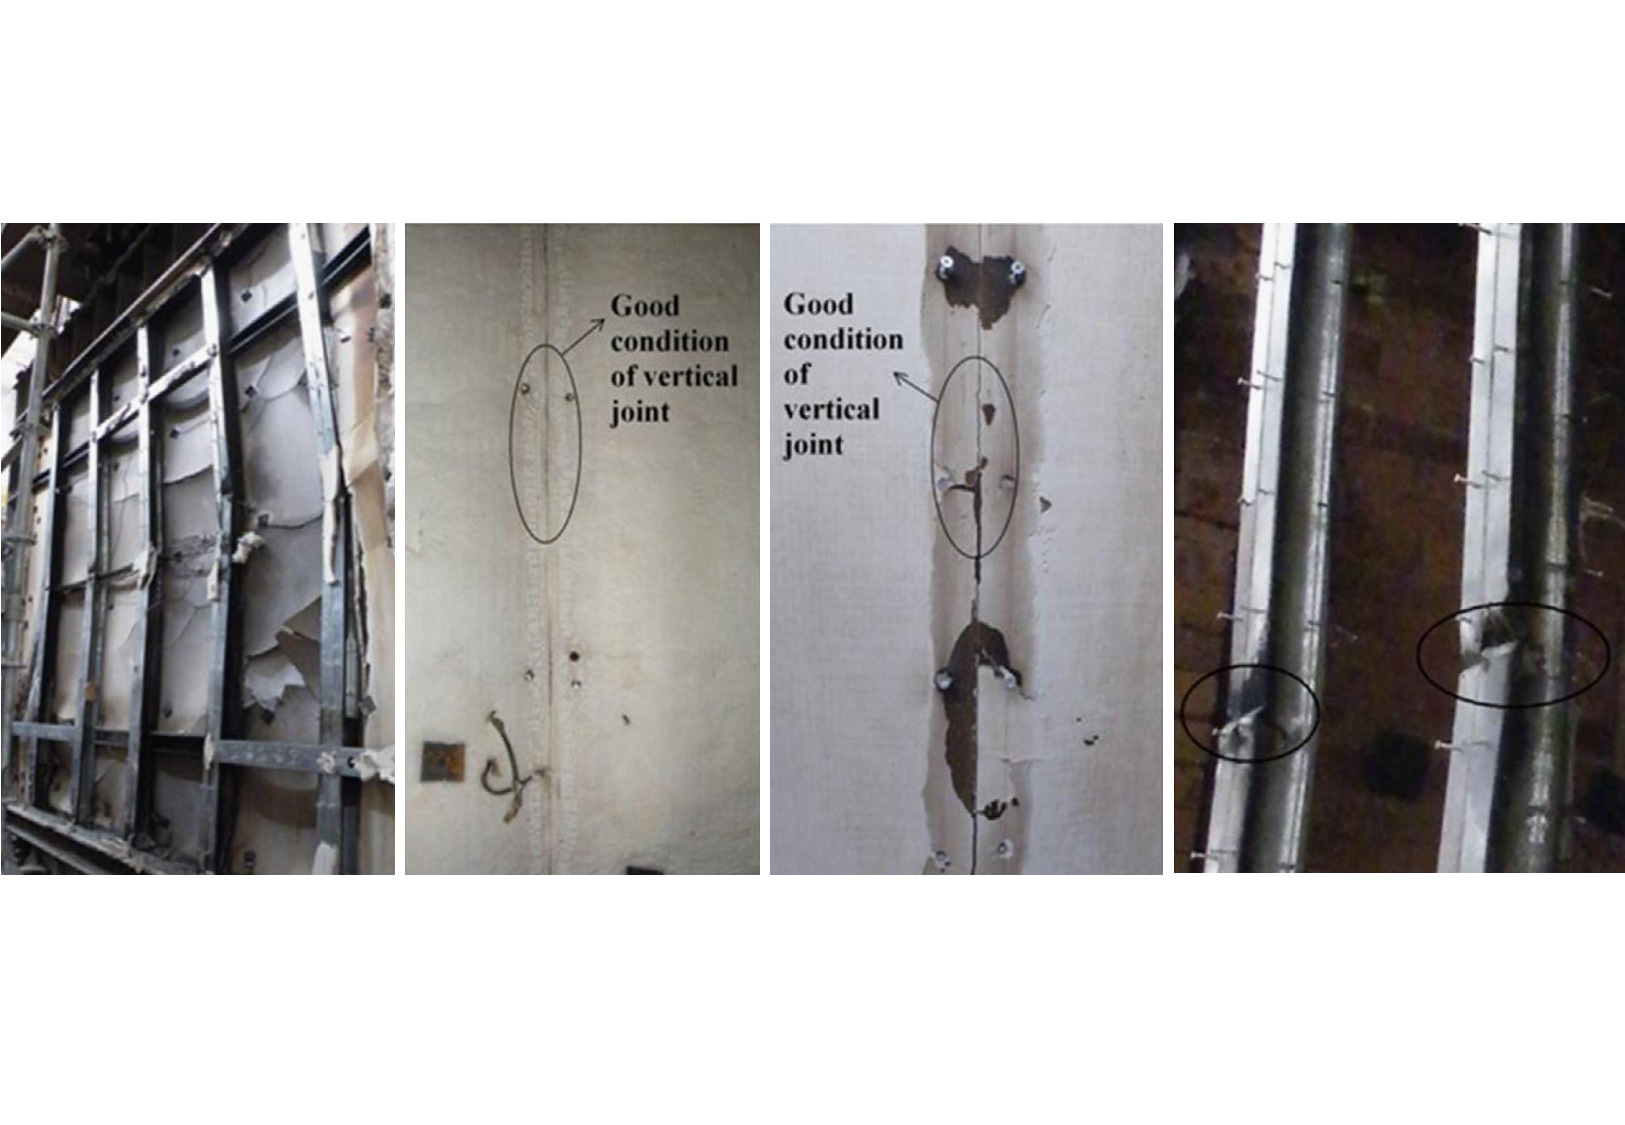
\includegraphics[width=14cm,height=5cm]{chen2013_test}		
		\caption{Lipped Channel Stud (LCS) failure in the fire test of \citet{Chen2013}}
		\label{fig:chen2013_test}
\end{figure}
Fire test results showed that the FRL will decreased with increasing in load ratio. The failure modes of the studs in the test walls with Bolivian magnesium board were different in comparison with other type of lining boards. Gypsum boards and bolivian boards were found to be less suitable for use in external walls due to durability resons, whereas ALC boards are preferred to be used in external walls. Increased screw-to-panel edge distance reduced the collapse of boards thereby preventing board open up on the fire side and cracks on the ambient side. 

\citet{Kolarkar2014} investigated the fire performance of gypsum plasterboards and composite panels. Fifteen small scale tests with 13 and 16 mm plasterboards were considered in their experimental investigation. Glass fibre, rock fibre and cellulose fibre insulations with different thickness and density were used as external insulation in the small scale LSF wall panels and their fire performance was investigated. It was found that, the composite wall panels in which the insulations were provided externally, performed better under fire exposure when compared to wall panels with cavity insulations. Another important observation is that the glass fibre insulation disintegrates at about 700\degree C, which is achieved at about 50 minutes of fire exposure resulting in premature failure of the walls with cavity insulation when compared with walls without cavity insulation. The cellulose fibre insulation resulted in better fire performance, provided low density cellulose is used when spraying the insulation within the cavity. Also, the process of spraying cellulose insulation within the cavity was not uniform always and could lead to varying results. Out of all the combinations used in this research, the rockwool external insulation was found to withstand disintegration better when compared with its counterparts. This is because the rockwool insulation did not disintegrate till end of the fire test, whereas other insulation materials disintegrated easily which ultimately reduced the FRL. 

\citet{Ariyanayagam2014e} studied the thermal performance of LSF walls under realistic design fires. Their test results were compared with those from LSF walls tested with standard ISO fire curve. Finite element models were developed for transient and steady state analyses and the results were compared with the test results. The FEA results for the realistic design fire curve were in good correlation with the experimental results. This research illustrated the difference between the effects caused by a standard fire and a realistic design fire in buildings. It also emphasized the use of realistic fire curves for the design of LSF walls. The effects of plasterboard joints and their arrangements were also investigated experimentally. It was observed that back blocking plasterboard joint arrangement used over the studs increased the FRL of LSF walls significantly by 25\% when compared with the traditional plasterboard joints. Numerical studies were also carried out to validate these results and were found to be in good correlation with experimental results. 

\citet{Kesawan2015} proposed the use of welded hollow flange channel (HFC) sections as studs in LSF walls. HFC sections have two flanges connected to the web through welding as shown in \Cref{fig:kesawan2015_test}. 
\begin{figure}[htbp]
	\centering
		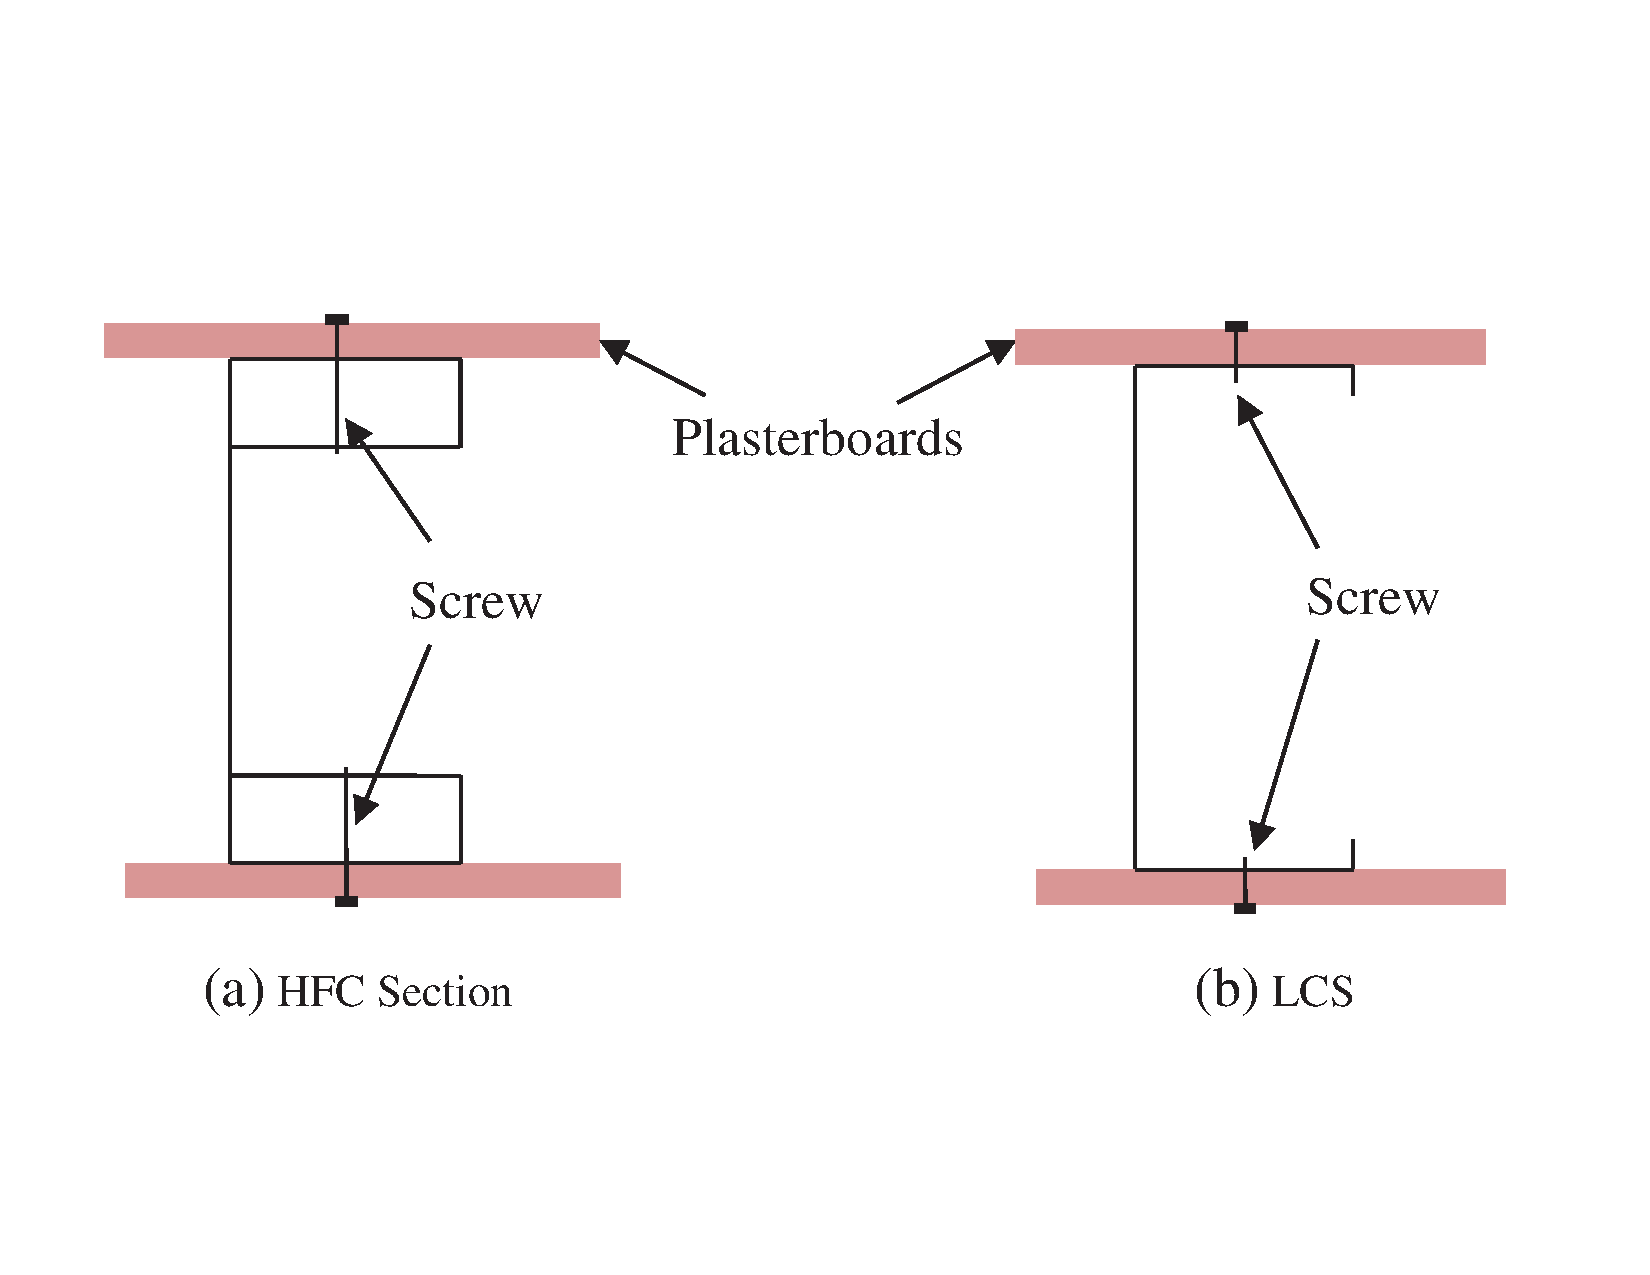
\includegraphics[width=10cm,height=5cm]{kesawan2015_section}		
		\caption{Hollow Flange Channel (HFC) studs used by \citet{Kesawan2015}}
		\label{fig:kesawan2015_test}
\end{figure}
Investigations were carried out on LSF walls with HFC stud sections to determine the thermal performance of LSF walls in fire. Initially the mechanical properties of the flange and web elements of the HFC sections were determined by tensile coupon tests at elevated temperatures. Secondly, full-scale fire tests of load bearing LSF walls with hollow flange channel studs were conducted. New parameters such as specific heat, density, emissivity and enthalpy were proposed for the thermal FE modelling of this new LSF wall configuration. The experimental investigation was carried out for various profiles of the HFC sections with and without insulations. Numerical models were created with measured mechanical properties and validated by comparing the results with experimental results. A numerical parametric study was conducted by varying the section geometry and stud thickness. Their results showed that the FRL was not improved by the stud section geometry, provided the section depth and thickness remain the same. 

\citet{Rusthi2017b} conducted full-scale fire tests of LSF walls using Australian Magnesium Oxide (MgO) boards instead of the conventional gypsum plasterboards with lipped channel sections. This research investigated the thermal properties of the MgO boards in detail followed by full-scale fire tests. All the fire tests were conducted under non-load bearing conditions. TThree full-scale fire tests were conducted, which included, LSF walls with and without cavity insulation. Significant cracking sound were observed with cracks on the ambient side after 25 min of fire test. Heavy delamination and cracking of MgO boards was noticeable on the fire exposed side after the fire test. Integrity based failure was the mode of failure in all fire tests. Despite the usage of mortar in board joints that can withstand high temperature, the cracking of the joints during fire test could not be nullified. It was also found that the usage of noggings in LSF walls with MgO boards, resulted in more cracking in comparison with wall assemblies without noggings. Therefore, it was recommended to exclude noggings in LSF walls subjected to large deformations.

\citet{Rusthi2017} developed heat transfer models in ABAQUS to predict the thermal behaviour of LSF walls under fire. 3D solid heat transfer brick elements were used for steel studs and plasterboards to create the heat transfer model. Tie constraints were used in the model to fix the steel studs and plasterboards for the heat transfer analysis. Five different LSF wall configurations were considered for the purpose of validation. Limiting hot flange temperatures proposed by \citet{Gunalan2013e,Ariyanayagam2014e} were considered in the parametric study to determine the failure times of the considered LSF wall configurations. The limiting hot flange temperatures were found to be decreasing with the increase in load ratio. The boundary conditions for the heat transfer model included the following.
\begin{itemize}
	\item ISO 834 standard time-temperature curve on the fire exposed side of the model.
	\item The model was enclosed on all the sides and cavity radiation was specified within the cavity with an emissivity co-efficient of 0.9.
	\item Convective film transfer coefficient of 10 $W/m^2/$\degree C was specified on the ambient surface while 25 $W/m^2/$\degree C was specified on the fire exposed surface.
	\item Radiation was assumed to be the dominant mode of heat transfer within the cavity, neglecting the effects of convection within the cavity.
\end{itemize}
Time-temperature curves were extracted from the thermal analysis and compared against the corresponding experimental results. The model predictions were found to exhibit reasonable match with the time–temperature curves from the experiments.

\citet{Ariyanayagam2018a} conducted five full-scale tests to investigate the fire performance of non-load bearing LSF walls. Gypsum plasterboard thicknesses of 13 and 16 mm were used along with 92 mm deep lipped channel studs. Test wall configurations included different plasterboard layers, cavity insulation and noggings to investigate the influence of these components on the fire performance of non-load bearing LSF walls. The test results showed that the typical failure mode in the non-load bearing LSF wall fire tests was insulation criterion, where the ambient surface plasterboard temperatures exceeded the limiting temperature. Finding from the research showed that the increase in plasterboard thickness resulted in increased FRL. The presence of noggings in non-load bearing LSF walls did not significantly influence the thermal behaviour. However, this can have considerable contribution to the structural behaviour under load bearing conditions. It was also found that the melting point of the insulation material used should be higher to achieve higher FRL for non-load bearing walls. 

\citet{Ariyanayagam2018c} then investigated the effects of low strength steel studs subjected to fire under load bearing conditions. Full-scale fire tests were conducted under 0.4-0.6 load ratios. Material properties at elevated temperatures were obtained through experimental investigation for the low strength steel studs and a parametric study was conducted using ABAQUS. Structural FE analysis results showed that the use of low strength steel resulted in reduction of FRLs by 25\% in comparison with a similar LSF wall made of high strength steel. The critical hot flange temperatures were also lower due to the reduction in the mechanical properties of steel at elevated temperatures. It was found that the usage of appropriate elevated temperature mechanical property reduction factors in FE analysis is critical in predicting the FRL through numerical methods. 

\citet{Dias2018a} conducted an experimental investigation on the fire performance of LSF walls with steel sheathing under non-load bearing conditions. Small-scale fire tests were conducted on 1 m$\times$ 1 m LSF wall assemblies with 0.5 mm steel sheathing placed at different positions \Cref{fig:dias_configuration}. Steel sheathing was used in the internal cavity wall facing surface and also on the fire exposed and ambient surfaces. The entrapment of water molecules from gypsum plasterboard on to the steel sheets resulted in increased thermal performance under non-load bearing conditions.   
\begin{figure}
	\centering
		\begin{tabular}{cc}
			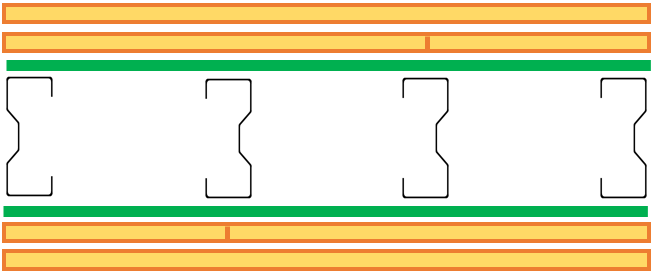
\includegraphics[scale=0.20]{double_pb_steel_in.PNG} &	
			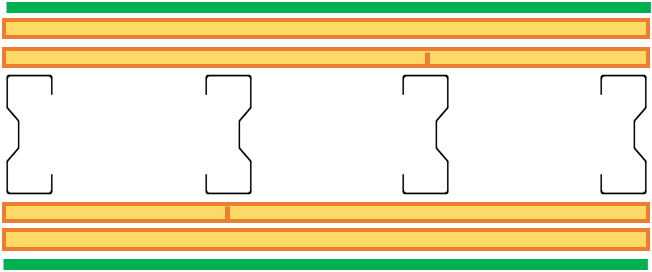
\includegraphics[scale=0.20]{double_pb_steel_out.PNG} \\
			(a) & (b) \\
		\end{tabular}
	\caption{Test configurations used by \citet{Dias2019c} (a) Internal and (b) External steel sheathing}
	\label{fig:dias_configuration}
\end{figure}
\begin{figure}[!htbp]
	\centering
		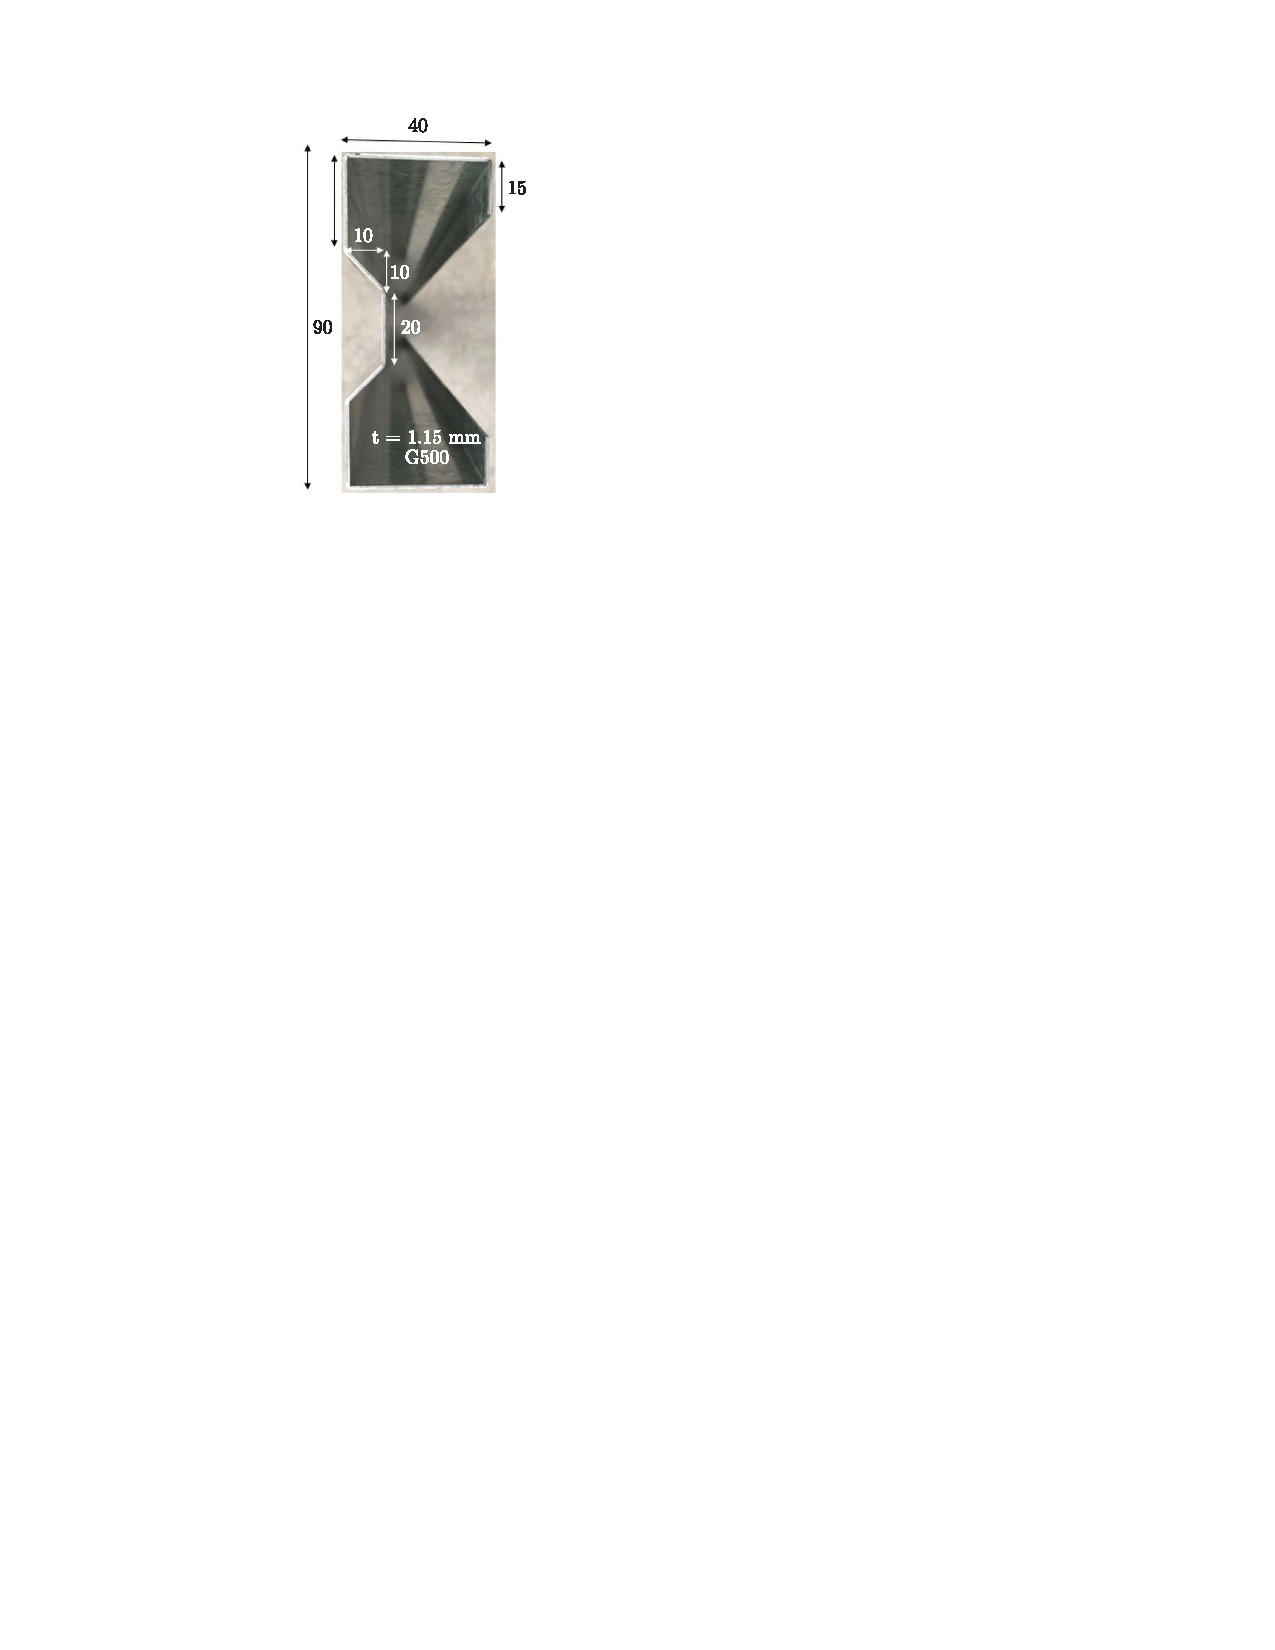
\includegraphics[width=6cm,height=7cm]{dias_stud}		
		\caption{Web-stiffened studs used by \citet{Dias2019c}}
		\label{fig:dias_stud}
\end{figure}

Later, \citet{Dias2019c} extended the investigation by conducting three full scale fire tests on LSF walls with steel sheathing. Web-stiffened studs were used instead of the conventional lipped channel sections (LCS) as shown in \Cref{fig:dias_stud}. The proposed new web-stiffened studs were able to withstand higher axial compression load in comparison with conventional LCS studs under ambient and fire conditions. However, when the FRL is considered based on the non-dimensional load ratios, these new wall configurations were found to provide only a marginal increase in the FRL in comparison with the conventional LSF wall configuration with LCS studs. 

\section{Thermal and Mechanical Properties of Cold-Formed Steels}

To study the behaviour of cold-formed steel structures under fire conditions, it becomes a necessity to account for the yield strength and elastic modulus values at elevated temperatures, as these parameters contribute to the structural strength of cold-formed steel members. The elevated temperature mechanical properties that are used in the research and design of cold-formed steel sections are based on BS EN 1993-1-3: (2006) and are shown in \Cref{tab:eurocode_reduction}. These mechanical properties with the corresponding reduction factors belong to hot-rolled steels and are also generally used for cold-formed steel sections. But \citet{Kankanamge2011} investigated this issue and proposed modified reduction factor equations for cold-formed steel sections. Tensile coupon tests were conducted under steady state conditions to study the behaviour of various grades cold-formed steels at elevated temperatures. The effect of creep was neglected in this study, as the experiments were concluded within an hour.

Specimen thicknesses of 1.50 and 1.95 mm with G250 and G450 steel grades and 0.95 mm thickness with G550 steel grade were used in their investigations. They also used the previous test results for cold-formed steel thicknesses upto 1 mm obtained by \citet{Ranawaka2009a} and developed suitable design equations for the yield strength and elastic modulus reduction factors of cold-formed steels at elevated temperatures $\Big(\dfrac{f_{y,T}}{f_{y,20}} \text{and} \dfrac{E_T}{E_{20}} \Big)$ as follows.

\begin{sidewaystable}[!htbp]
	\centering
	\caption{Reduction Factors for Cold-Formed Steels at Elevated Temperatures}
	\begin{tabular}{ccccc}
		\toprule
		\multirow{3}[6]*{\minitab[c]{Stud \\ Temperature}} & \multicolumn{4}{p{26.14em}}{Reduction factors at temperature $\theta$a relative to the value of fy or Ea at 20\degree C} \\
		\cmidrule{2-5}    \multicolumn{1}{c}{} & \multicolumn{1}{p{6.07em}}{Reduction factor (relative to $f_y$) for effective yield strength} & \multicolumn{1}{p{6.5em}}{Modified factor (relative to $f_y$) for satisfying deformation criteria} & \multicolumn{1}{p{6.355em}}{Reduction factor (relative to $f_y$) for proportional limit} & \multicolumn{1}{p{7.215em}}{Reduction factor (relative to $E_a$) for the slope of linear elastic range} \\
		\cmidrule{2-5} \multicolumn{1}{c}{} & \multicolumn{1}{p{6.07em}}{\textit{$k_y$$\theta$ = $f_y$,$\theta$/$f_y$}} & \multicolumn{1}{p{6.5em}}{\textit{$k_x$$\theta$ = $f_x$,$\theta$/$f_y$}} & \multicolumn{1}{p{6.355em}}{\textit{$k_p$$\theta$ = $f_p$,$\theta$/$f_y$}} & \multicolumn{1}{p{7.215em}}{\textit{$k_E$$\theta$ = $E_a$,$\theta$/$E_a$}} \\
		\midrule
		20 \degree C & 1    & 1    & 1    & 1 \\
		\midrule
		100 \degree C & 1    & 1    & 1    & 1 \\
		\midrule
		200 \degree C & 1    & 0.922 & 0.807 & 0.9 \\
		\midrule
		300 \degree C & 1    & 0.845 & 0.613 & 0.8 \\
		\midrule
		400 \degree C & 1    & 0.77 & 0.42 & 0.7 \\
		\midrule
		500 \degree C & 0.78 & 0.615 & 0.36 & 0.6 \\
		\midrule
		600 \degree C & 0.47 & 0.354 & 0.18 & 0.31 \\
		\midrule
		700 \degree C & 0.23 & 0.167 & 0.072 & 0.13 \\
		\midrule
		800 \degree C & 0.11 & 0.087 & 0.05 & 0.09 \\
		\midrule
		900 \degree C & 0.06 & 0.051 & 0.0375 & 0.0675 \\
		\midrule
		1000 \degree C & 0.04 & 0.034 & 0.025 & 0.045 \\
		\midrule
		1100 \degree C & 0.02 & 0.017 & 0.0125 & 0.0225 \\
		\midrule
		1200 \degree C & 0    & 0    & 0    & 0 \\
		\bottomrule
	\end{tabular}%
	\label{tab:eurocode_reduction}%
\end{sidewaystable}%

 \subsection*{Yield Strength for Low Strength Steels}
\begin{equation}
20 \leq T \leq 200\degree C , \dfrac{f_{y,T}}{f_{y,20}} = -0.0005T+1.01
\label{eq:yield_low1}
\end{equation}
\begin{equation}
200 \leq T \leq 800\degree C , \dfrac{f_{y,T}}{f_{y,20}} = 25(1.16-T^{0.022})
\label{eq:yield_low2}
\end{equation}
\subsection*{Yield Strength for High Strength Steels}
\begin{equation}
20 \leq T \leq 300\degree C , \dfrac{f_{y,T}}{f_{y,20}} = \Big\{ 1-\dfrac{(T-20)^{4.56}}{1*10^{10}T} \Big\}
\label{eq:yield_low3}
\end{equation}
\begin{equation}
300 \leq T \leq 600\degree C , \dfrac{f_{y,T}}{f_{y,20}} = \Big\{ 0.95-\dfrac{(T-300)^{1.45}}{7.76T} \Big\}
\label{eq:yield_low4}
\end{equation}
\begin{equation}
600 \leq T \leq 800\degree C , \dfrac{f_{y,T}}{f_{y,20}} = -0.0004T + 0.35
\label{eq:yield_low5}
\end{equation}
\subsection*{Elastic Modulus for Low and High Strength Steels}
\begin{equation}
20 \leq T \leq 200\degree C , \dfrac{E_T}{E_{20}} = -0.0008355T+1.0167
\label{eq:yield_high1}
\end{equation}
\begin{equation}
200 \leq T \leq 800\degree C , \dfrac{E_T}{E_{20}} = -0.00135T+1.1201
\label{eq:yield_high2}
\end{equation}
\citet{Kankanamge2011} improved the elevated temperature stress-strain models developed by \citet{Ranawaka2009} for cold-formed steels by the following equation. 
\begin{equation}
\epsilon_T = \dfrac{f_T}{E_T} + \beta \Big(\dfrac{f_{y,T}}{E_T}\Big)\Big(\dfrac{f_T}{f_{y,T}}\Big)^{\eta_{T}}
\label{eq:yield_high3}
\end{equation}
For high strength steels (G550), 20$ \leq$ T $\leq$ 800\degree C,
\begin{equation}
	\eta_T = -3.05 \times 10^-7 T^3 + 0.0005T^2 - 0.2615T + 62.653
	\label{eq:yield_high4}
\end{equation}
\begin{equation*}
\beta=0.86
\end{equation*}
		
For low strength steels, 300$ \leq$ T $\leq$ 800\degree C,
\begin{equation}
\eta_T = 0.000138T^2 - 0.085468T + 19.212
\label{eq:yield_high5}
\end{equation}
\begin{equation*}
	\beta=1.5
\end{equation*}

This research concluded that steel grade influences the yield strength at elevated temperatures. However, there was no effect on the yield strength with respect to thickness of steel. The proposed equations predicted the mechanical properties with good accuracy for low and high-grade cold-formed steels. All these equations (\Cref{eq:yield_low1,eq:yield_low2,eq:yield_low3,eq:yield_low4,eq:yield_low5,eq:yield_high1,eq:yield_high2,eq:yield_high3,eq:yield_high4,eq:yield_high5}) are now included in Section 9 of AS/NZS 4600 \citet{ASNZ4600}.

\section{Thermal Properties of Plasterboard}

Gypsum plasterboards are widely used in the construction of walls in Australia and throughout the globe. Like other materials, gypsum plasterboards provide resistance to fire, but through time several industries have come up with improved plasterboards capable of resisting fire. But to predict the thermal performance of LSF wall systems the thermal properties of plasterboards are needed. Thermal properties include conductivity, specific heat, mass loss etc. Many studies were conducted to determine the thermal properties of gypsum plasterboard and are discussed next.

The effect of moisture transfer at high temperatures on the specific heat of gypsum plasterboard was investigated by \citet{Ang2009}. Numerical techniques and experimental methods were used to investigate the effects of moisture transfer on specific heat when gypsum plasterboards were exposed to fire. The equivalent energy required at higher temperatures for the water to evaporate from the plasterboard was not known. Therefore, an approximate temperature of 100\degree C was assumed for the initial trials. Apart from ablation, shrinkage and collapse of the plasterboards under fire as reported by \citet{Jones2001}, the size and the loading conditions were found to affect the specific heat. In this study the effects of ablation, shrinkage and collapse were neglected. Combined heat and mass transfer was the modelling technique adopted in this study. To solve this heat transfer problem, thermal and pressure boundary conditions were considered in the model. Computer program called HEATMASS was developed based on the laws of heat and mass transfer. Additional inputs such as porosity and permeability along with normal heat transfer analysis inputs such as specific heat, density and thermal conductivity of plasterboard were used. It is to be noted that gypsum contains 3\% free water and 21\% chemically bound water as per \citet{Mehaffey1994}. This water content is responsible in preventing fire from spreading to the other side of the board. At higher temperatures, the plasterboard calcinates and the water is lost from the plasterboard resulting in plasterboard fall-off during fire exposure. Experimental investigations were conducted to determine the saturated permeability of gypsum plasterboard. It was assumed that, the permeability of gypsum remains unchanged at high temperatures due to the micro nature of the particles, thereby resulting in micro-cracks. It was concluded that the appropriate value of permeability of gypsum plasterboard was 5 $\times$ 10$^{-9}$ m/s. This was derived by validating the experimental results with the numerical model in HEATMASS. It was also found that the specific heat for numerical analysis is a function of gypsum plasterboard's permeability. It was also proposed that a modification factor of 1.45 along with the permeability in standard fire condition is to be included to achieve good agreement in the numerical analysis. 

\citet{Kontogeorgos2011} investigated the thermal performance of gypsum plasterboard at various dehydration temperatures. Past research studies showed that the first dehydration of gypsum plasterboard occurs at around 150\degree C. In this study the thermal conductivity, specific heat and density were measured as a function of the dehydration temperature i.e. until 300\degree C. Relationship between the dehydration energy as a function of mass loss during dehydration process was also investigated. Different heating rates were used in determining the thermal propertied of gypsum plasterboard. Specimen sizes of 200 $\times$ 150 $\times$ 20 mm and 160 $\times$ 40 $\times$ 40 mm were used. Thermocouples were fixed on eight different locations in the specimen and the temperature was recorded at 2 s intervals. 
\begin{figure}[htbp]
	\centering
		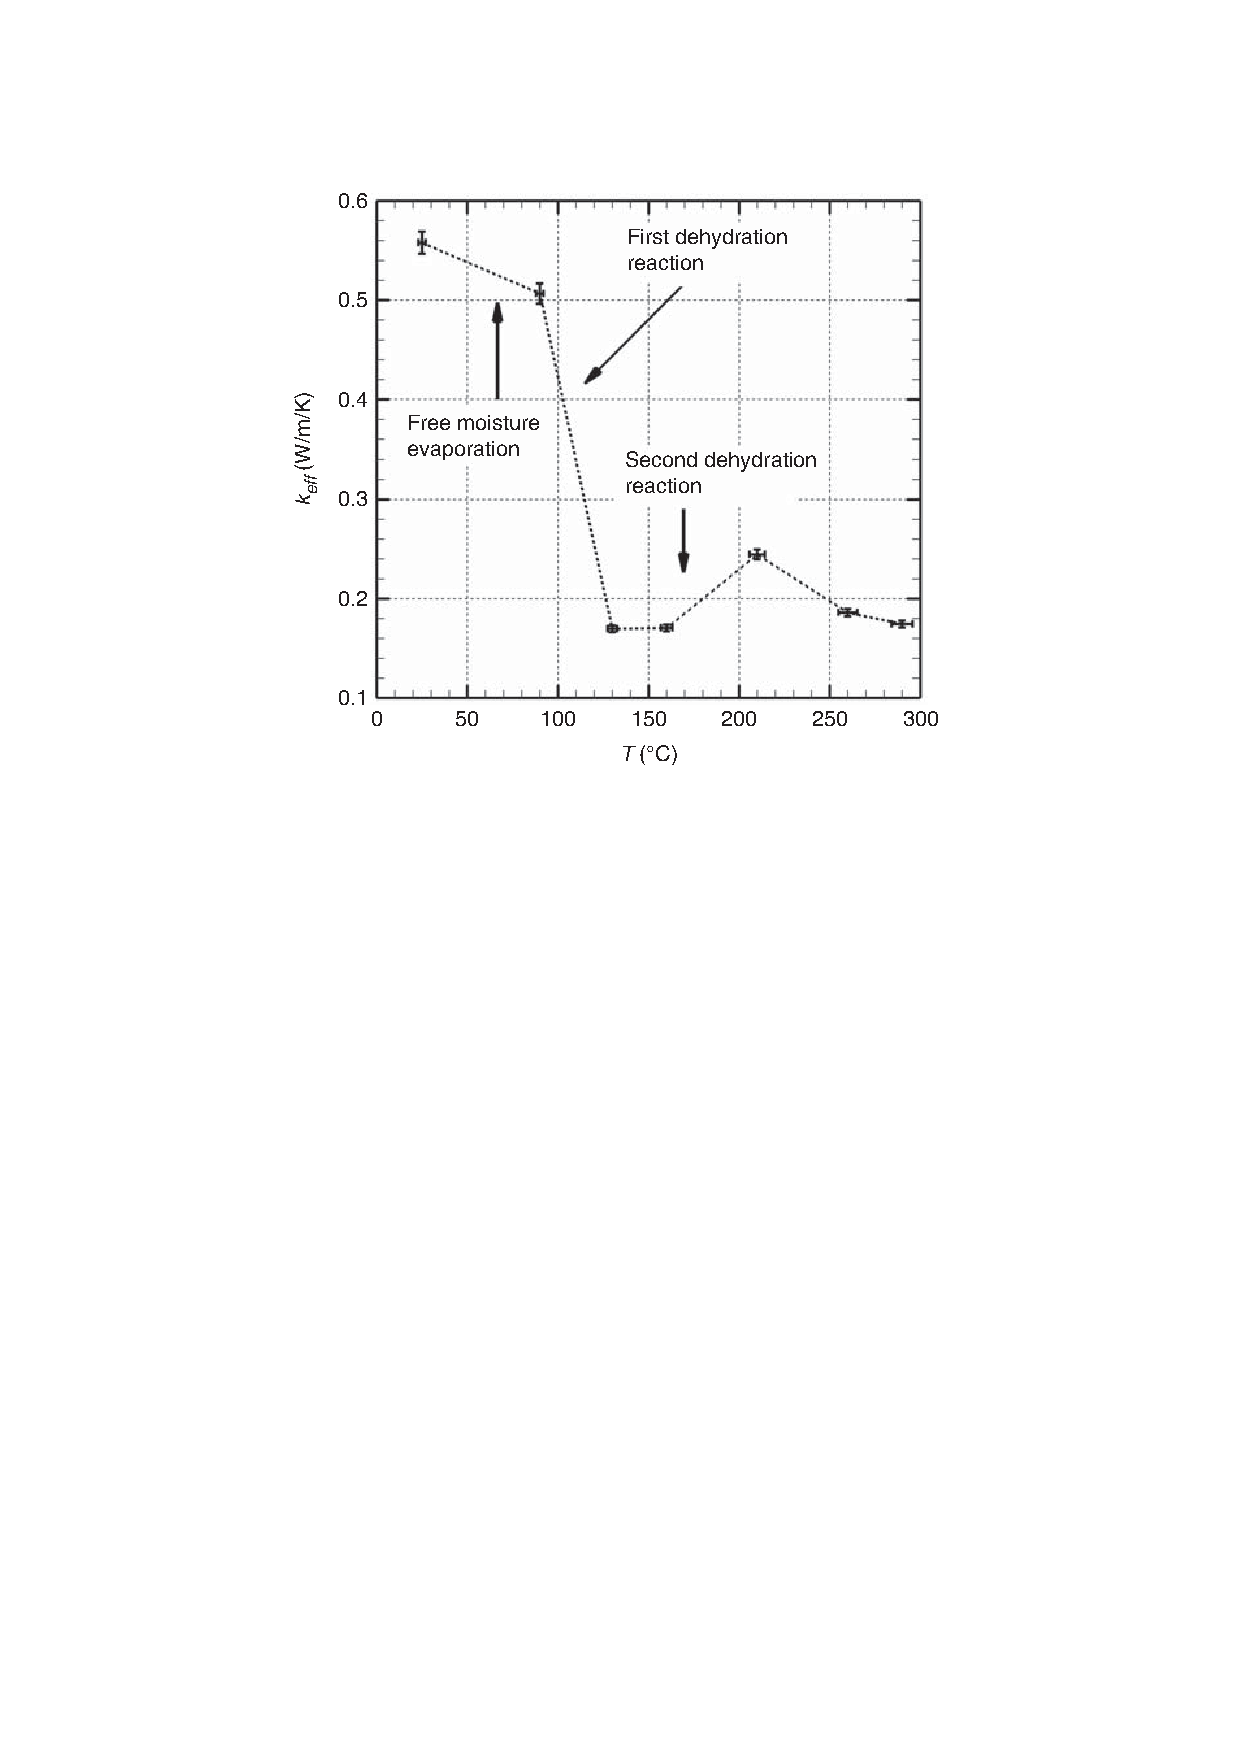
\includegraphics[width=6cm,height=5cm]{kontogeorgos_conductivity}		
		\caption{Thermal conductivity used by \citet{Kontogeorgos2011}}
		\label{fig:kontogeorgos_conductivity}
\end{figure}

Hot wire method was used to measure the thermal conductivity of the specimen. This method is based on the transient method of heat transfer as per ISO 8894-1 (2010) (latest amendment). OHAUS scale was used to measure the weight of the samples exposed to elevated temperatures and to calculate the mass loss. The energy required for dehydration was calculated using Differential Scanning Calorimetry (DSC) at a heating rate of 20\degree C/min using airflow from 0 \degree C to 600\degree C. The thermal conductivity as a function of temperature obtained from the experiments is shown in \Cref{fig:kontogeorgos_conductivity}.This investigation concluded that due to the evaporation of free moisture content at about 100\degree C, the thermal conductivity decreases after the first dehydration point. Also, it provided an experimental method to predict the energy absorbed by the gypsum plasterboard at dehydration point when exposed to elevated temperatures.

\section{Numerical Simulation}

\citet{Sultan1996} proposed a one-dimensional mathematical model to predict the heat transfer in non-load bearing and non-insulated LSF walls. Single row of steel studs spaced at 600 mm centres and 0.45 m thick were considered. To reduce the complexity of the analysis the radiative heat transfer from the studs to the plasterboards was ignored. Also the moisture movement and cracking of the plasterboards were not considered. Time-Temperature profile from CAN/ULC-S 101-M89 was adopted for the model based on ASTM 119-16 (2016).

\begin{equation} \label{eq:sultan1996}
T_f = T_\infty + 750 [1-exp(-3.79553)\sqrt{\tau}] + 170.41\sqrt{\tau}
\end{equation}

Where
\begin{description}[itemsep=0pt,parsep=0pt]
	\item $T_f$ = Temperature of fire curve (source) (\degree K);
	\item $T_\infty$ = Temperature of Ambient side;
	\item $\tau$ = time, h.
\end{description}
The heat transfer through the wall from the fire side to the ambient side was governed by the basic heat transfer equations of conduction, convection and radiation. The emissivity of the plasterboard was kept constant at 0.8 throughout the model. The convective heat transfer co-efficient was varied for different faces such as the fire exposed face, wall cavity and the unexposed face of the LSF wall as in \Cref{eq:hexp,eq:hcav,eq:huexp}.

\begin{equation}\label{eq:hexp}
h_{exp} = 0.95{(T_f - T_g)}^{0.33}
\end{equation}

\begin{equation}\label{eq:hcav}
h_{exp} = 0.95{(T_f - T_g)}^{0.33}
\end{equation}

\begin{equation}\label{eq:huexp}
h_{uexp} = 1.42{(T_g - T)}/L^{0.33}
\end{equation}

Where
\begin{description}[itemsep=0pt,parsep=0pt]
	\item $ h_{exp} $ = Convective heat transfer co-efficient (fire exposed side)
	\item $ h_{cav} $= Convective heat transfer co-efficient (cavity) 
	\item $ h_{u exp} $ = Convective heat transfer co-efficient (unexposed side) 
	\item $ T_f $ = Temperature of fire curve (source) (\degree K)
	\item $ T_g $ = Temperature of gypsum board (\degree K)
	\item $T$ = Temperature (\degree K)
	\item $L$ = Wall height (m)
	\item $d$ = Wall cavity depth (m)
\end{description}
Finite difference method was adopted to predict the temperature history across the wall and corresponding equations were proposed for different locations of the wall because of the varying boundary conditions. To validate the mathematical model, small-scale fire tests of specimens 1 m $\times$ 1 m and 1 m $\times$ 2 m were conducted with the same configuration adopted in the mathematical model. The failure criteria for the fire test were in accordance with CAN/ULC-S 101-M89. The heat transfer mechanism in the fire test within the cavity was through natural and forced convection at different time of fire exposure and through radiation. This was not considered in the mathematical model. This research work resulted in clear insight of the heat transfer mechanisms across the LSF wall assembly. 

\citet{Keerthan2012a} conducted numerical studies of gypsum plasterboard panels. The thermal inputs such as thermal conductivity, specific heat, relative density and mass loss for the numerical analysis were derived through thermal property test conducted on gypsum plasterboards. From the past research conducted on gypsum plasterboards by \citet{Mehaffey1994,Sultan1996} and other researchers, it is evident that the plasterboard when exposed to fire above 800\degree C as per the ISO 834 standard fire curve will not stay intact. So apparent thermal conductivity values were used in the numerical models after 800\degree C. This is because, the plasterboard cracks after this temperature letting the hot gases to pass through, which cannot be predicted by the numerical model. The thermal conductivity, specific heat and relative density of plasterboards obtained from past research are shown in Figures \ref{fig:keerthan_pbprop} (a) to (c). Since there were discrepancies in the specific heat peak values, second dehydration point and relative density of plasterboards measured by past research works, experiments were carried out by \citet{Keerthan2012} using differential scanning calorimetry (DSC) and thermo gravimetric analysis (TGA). From the DSC heat flow data, specific heat was calculated as per ASTM E1269 (2011). Their experimental results for specific heat, relative density and the proposed idealised thermal conductivity are shown in Figures \ref{fig:keerthan_measured} (a) to (c).

\begin{figure}[htbp]
	\centering
		\begin{tabular}{c}
			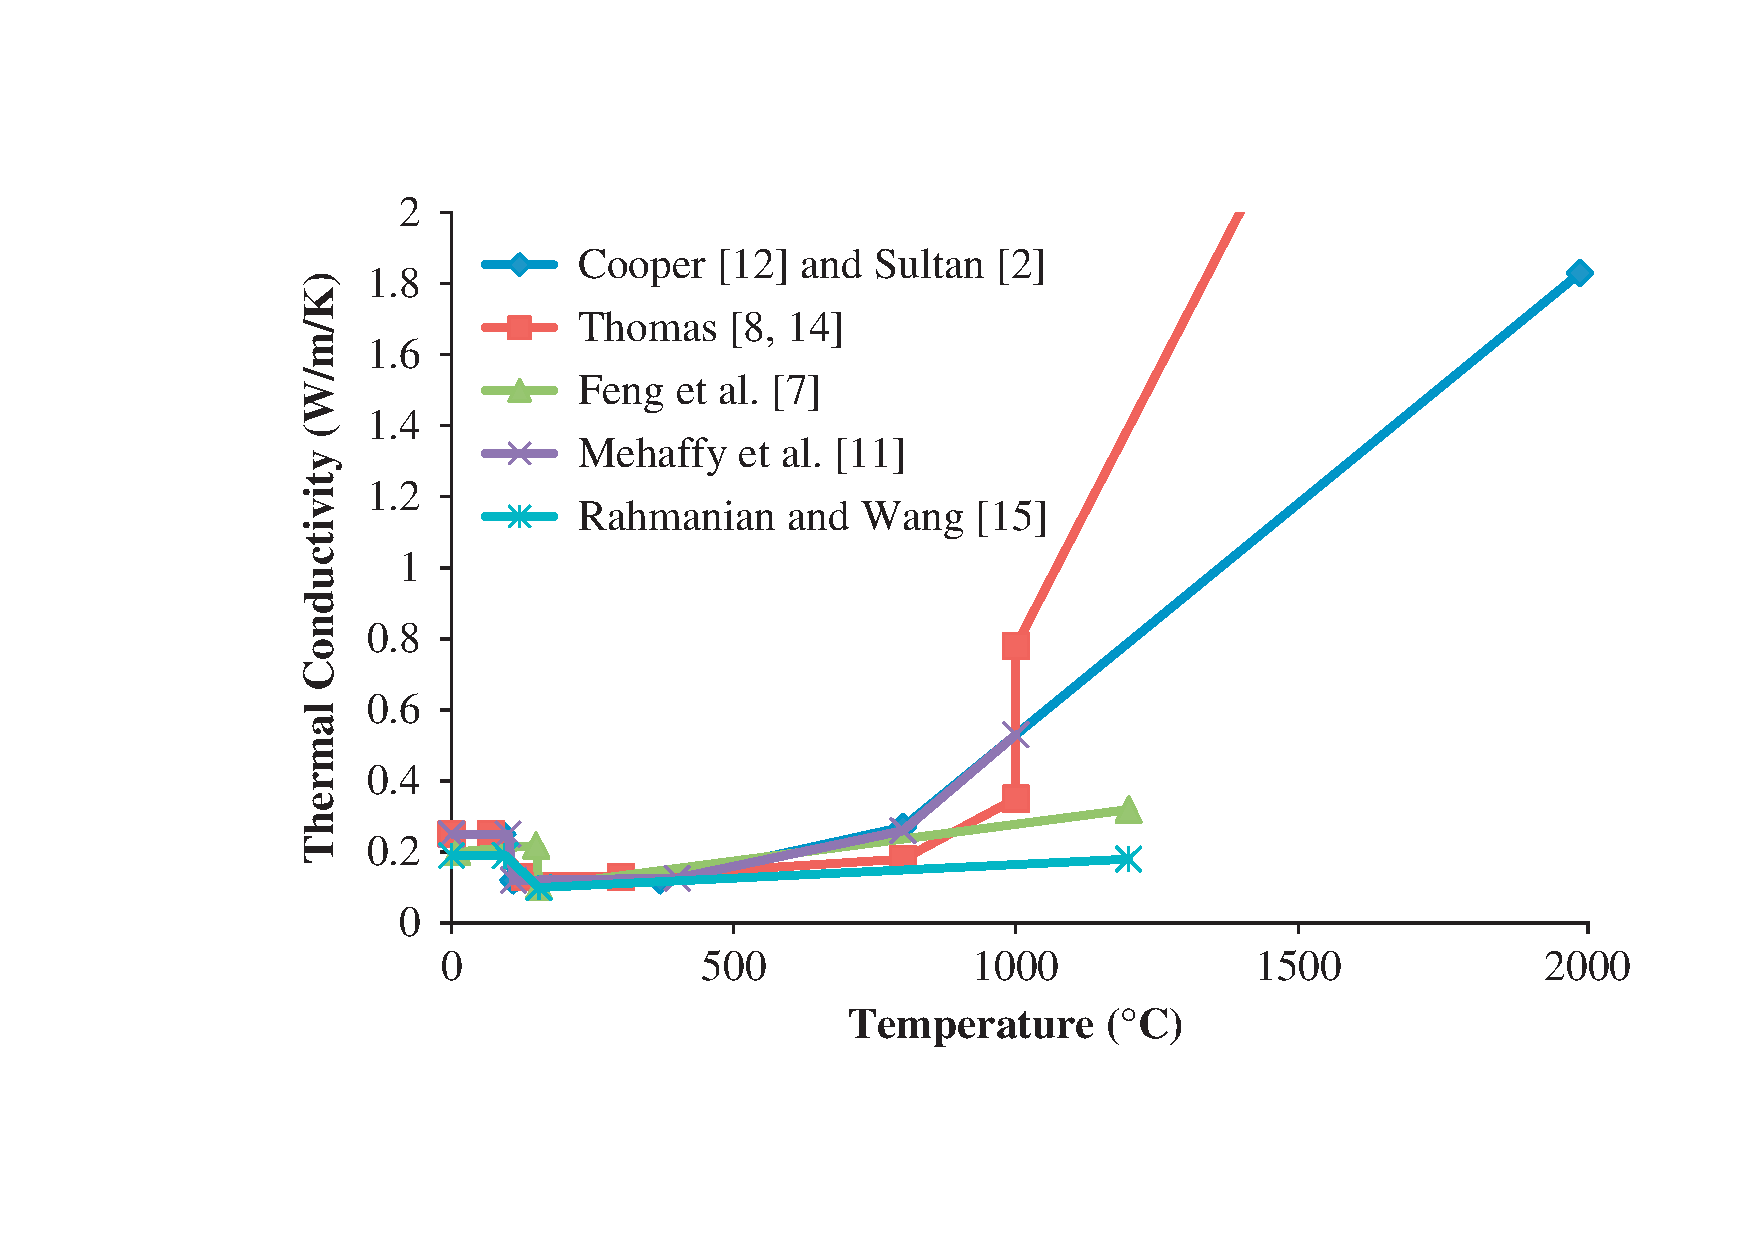
\includegraphics[width=8.5cm,height=6cm]{keerthan_conductivity.pdf} \\
			(a) \\
			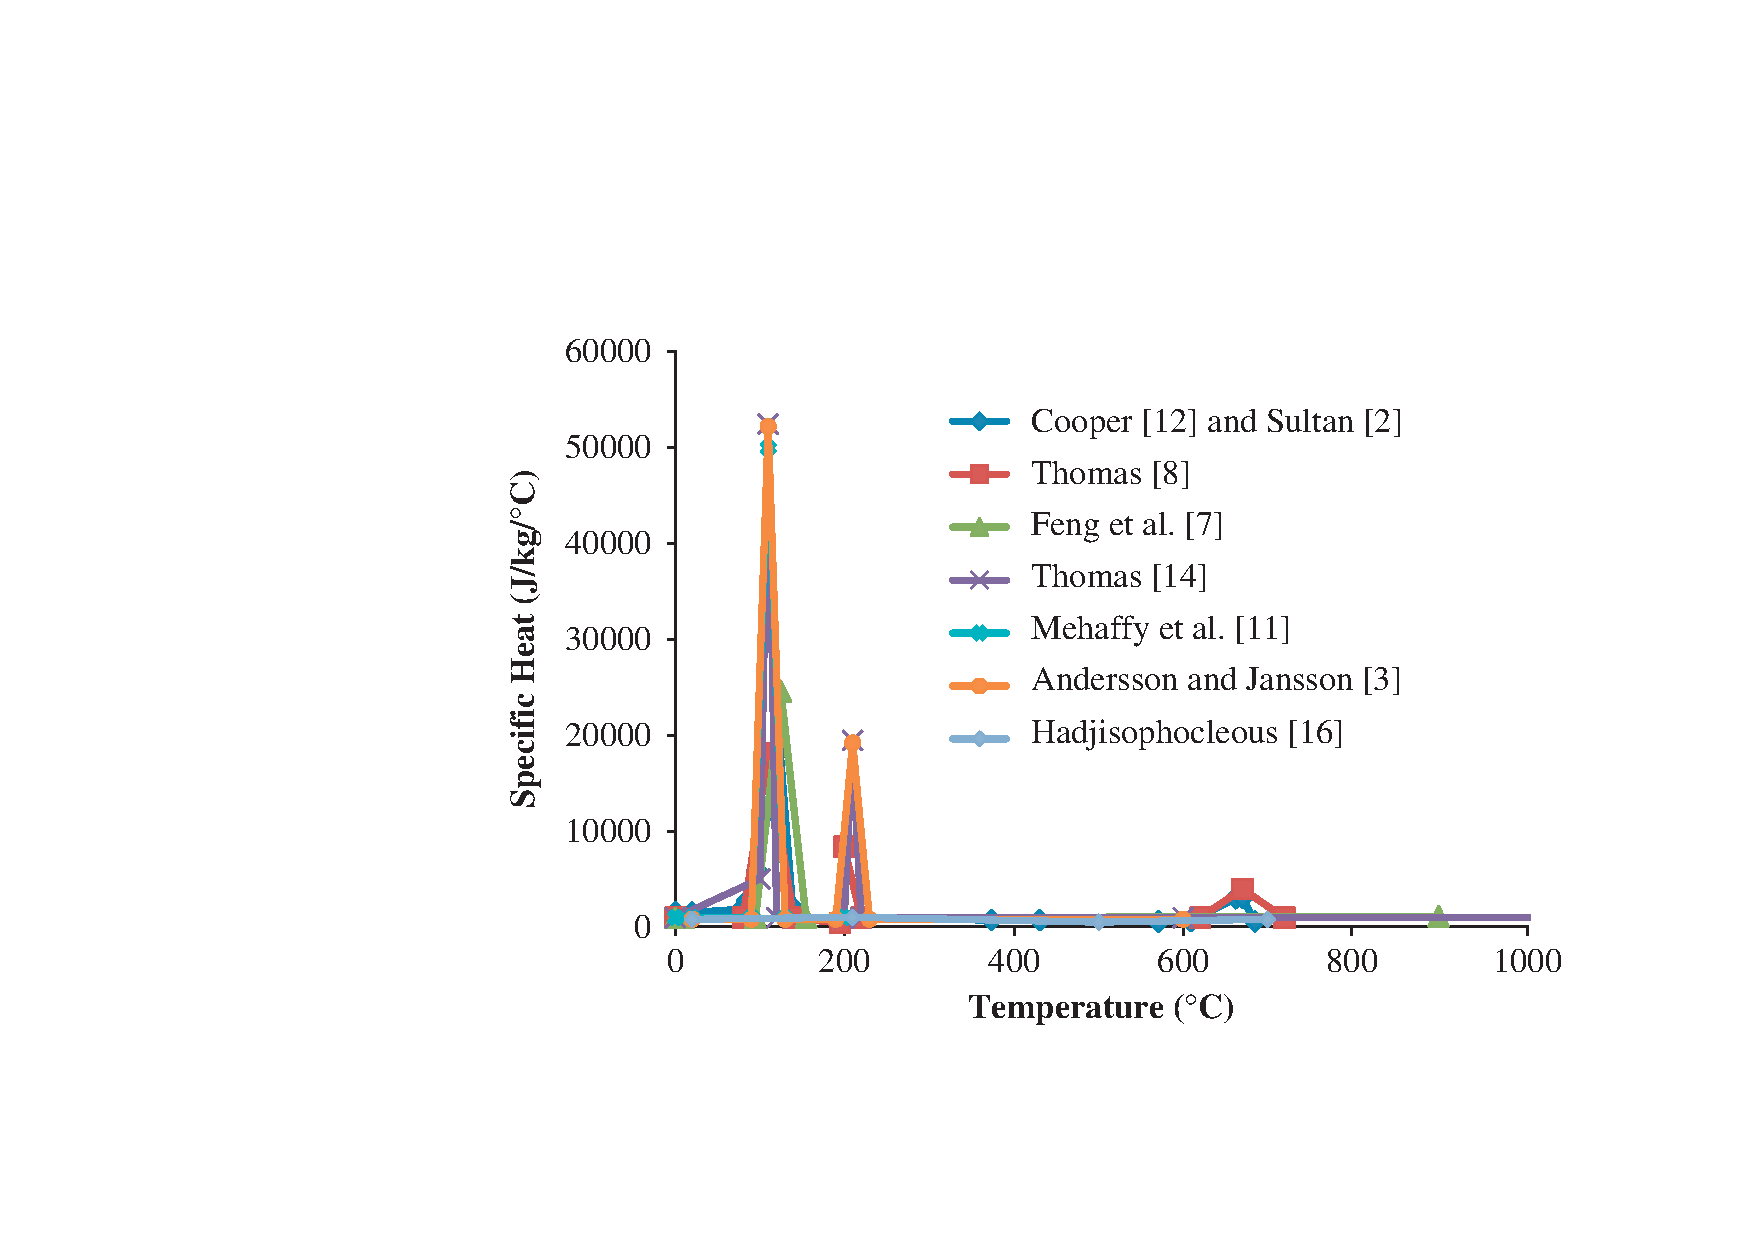
\includegraphics[width=8.5cm,height=5.5cm]{keerthan_cp.pdf} \\
			(b) \\ 
			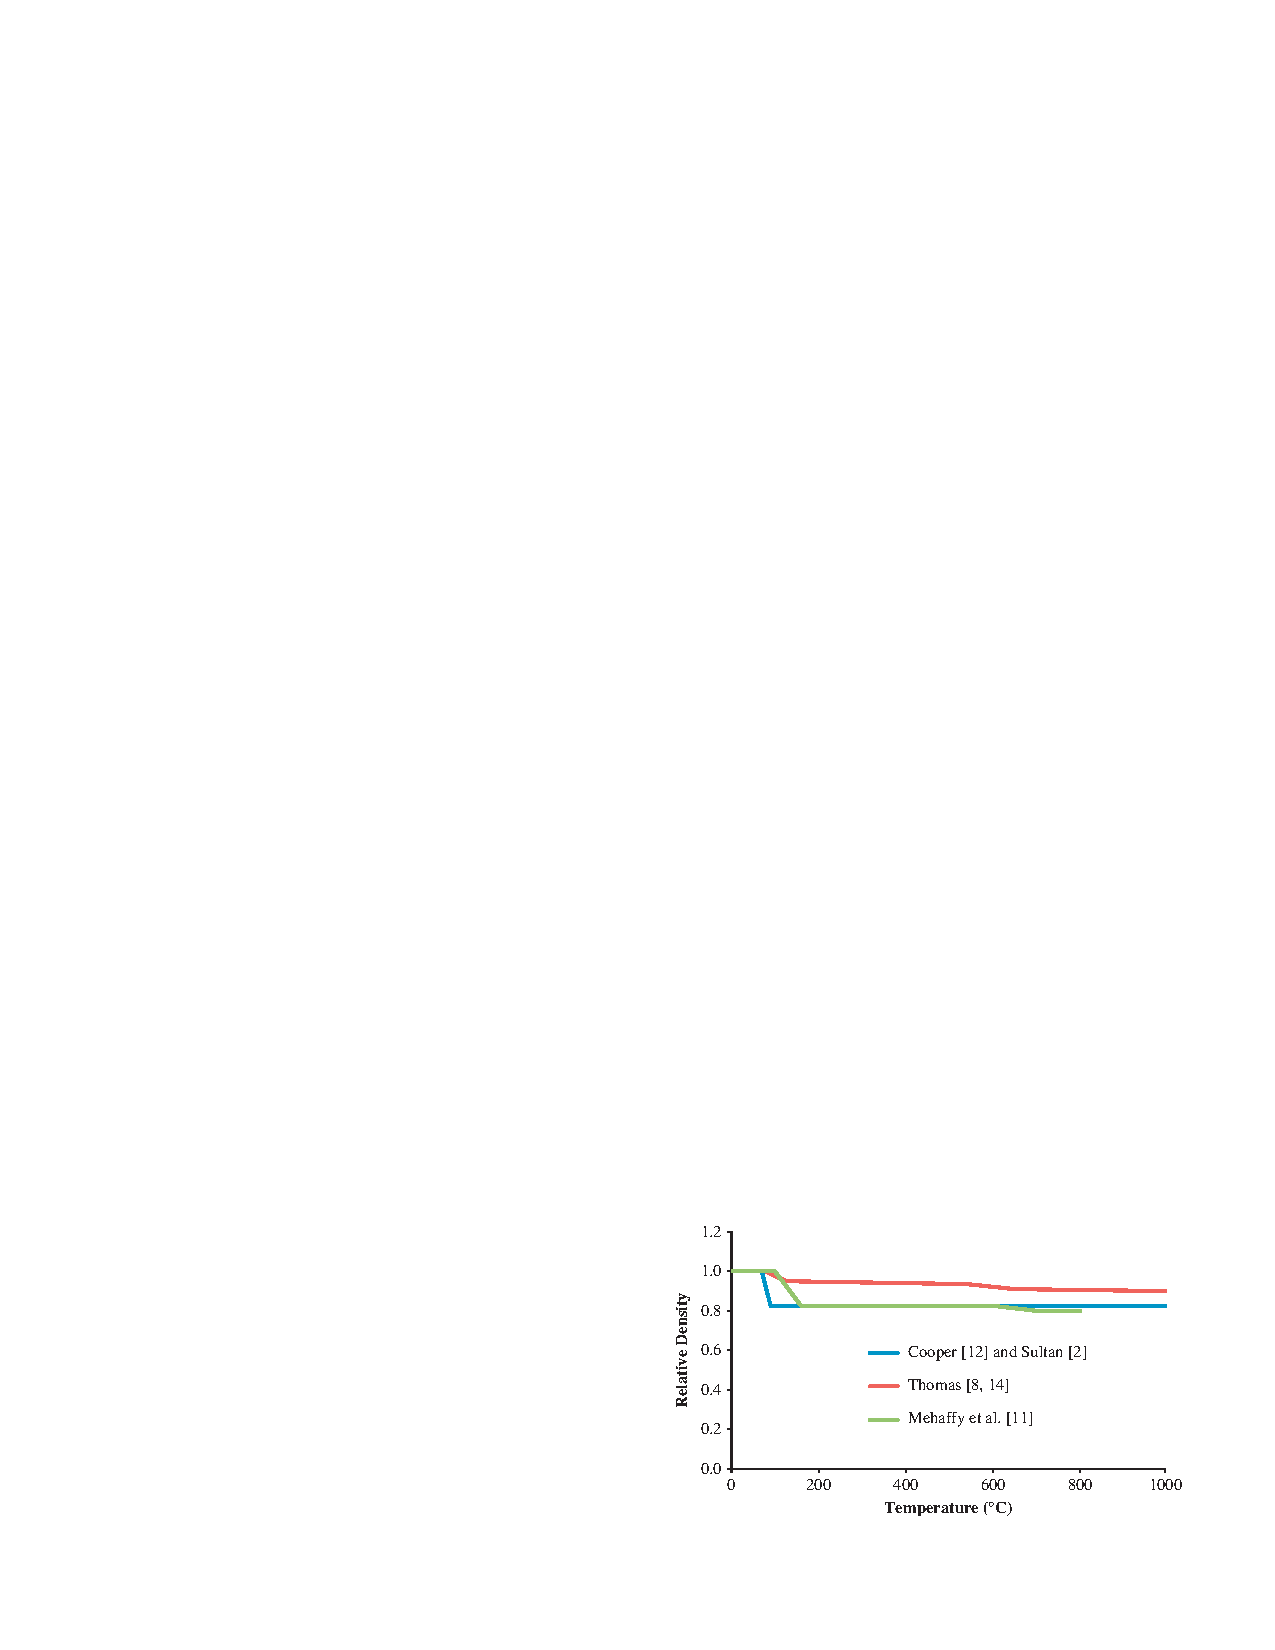
\includegraphics[width=8.5cm,height=5.5cm]{keerthan_density.pdf} \\
			(c) \\
		\end{tabular} 
		\caption{Thermal properties of plasterboard from \Citet{Keerthan2012a}}
		\label{fig:keerthan_pbprop}
\end{figure}

\begin{figure}[htbp]
	\centering
		\begin{tabular}{c}
			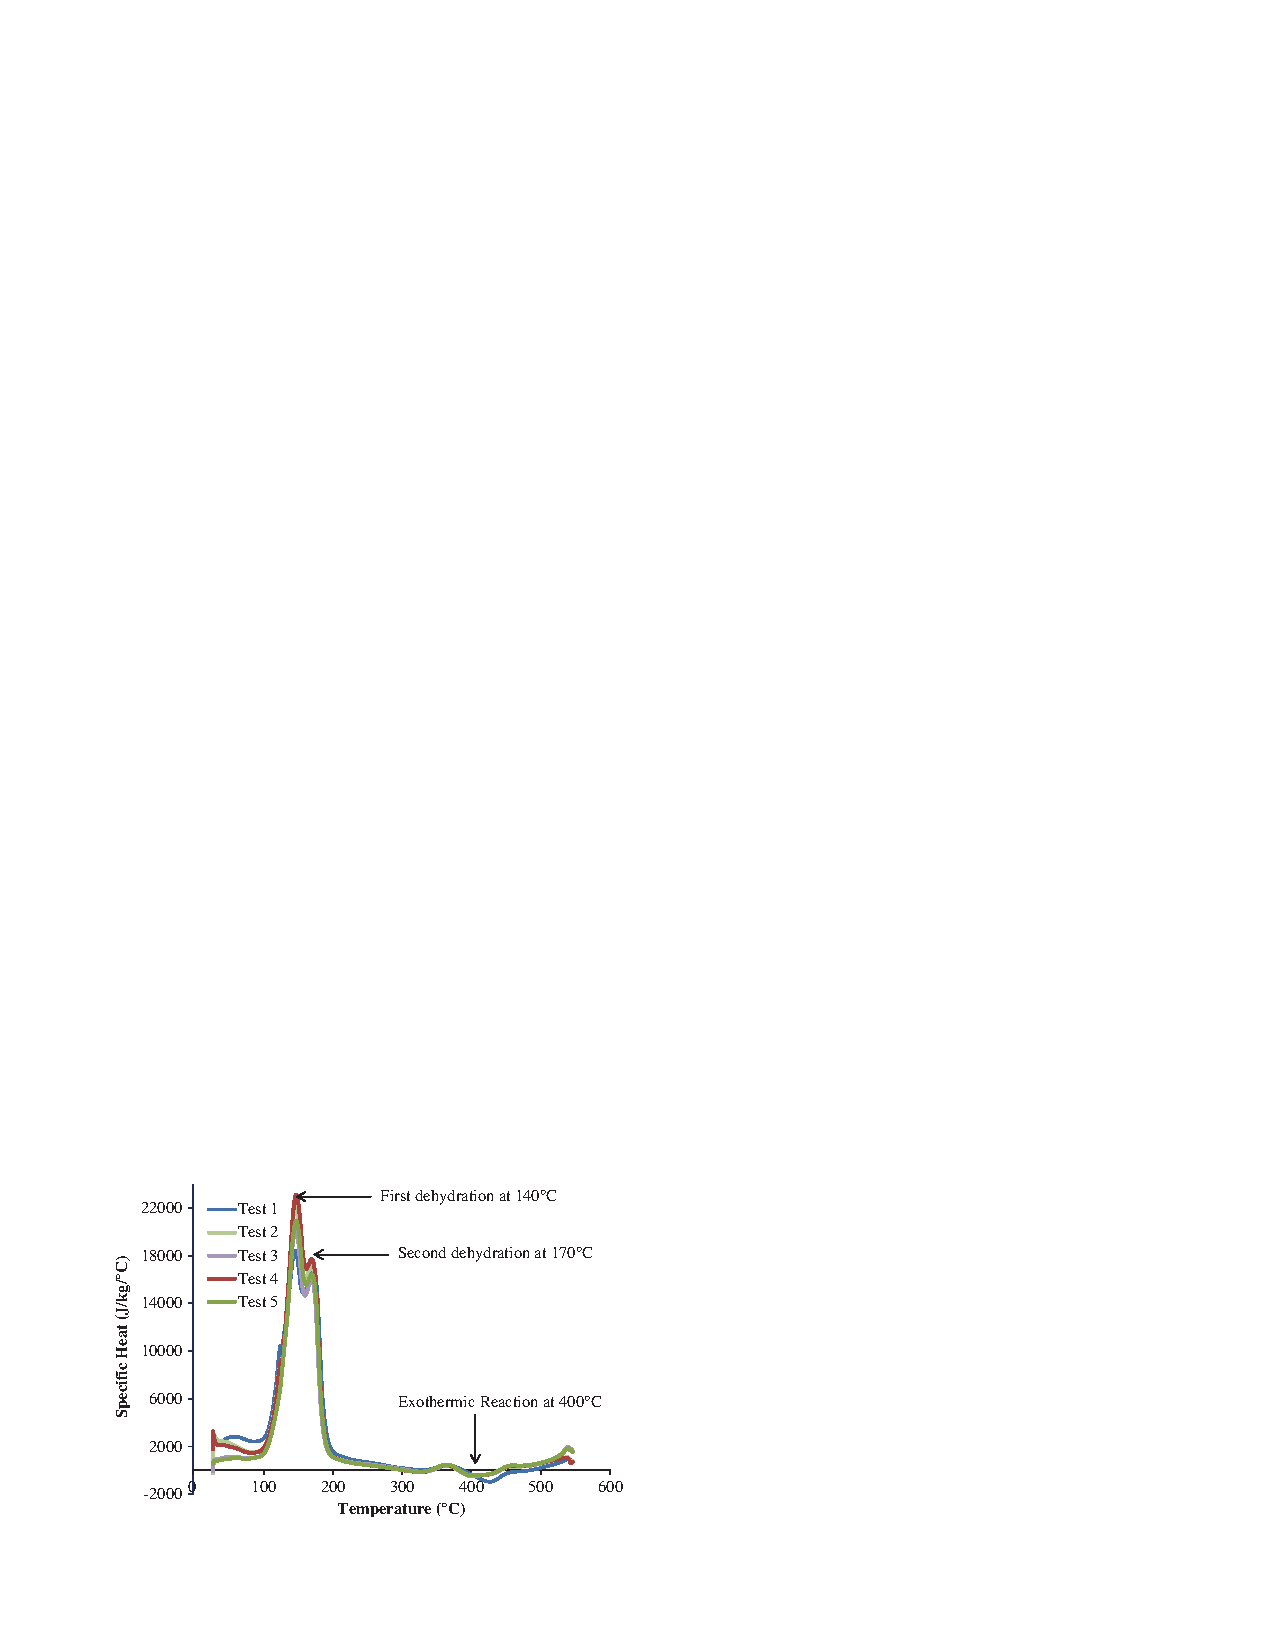
\includegraphics[width=8.5cm,height=6cm]{keerthan_cp_measured.pdf} \\
			(a) \\
			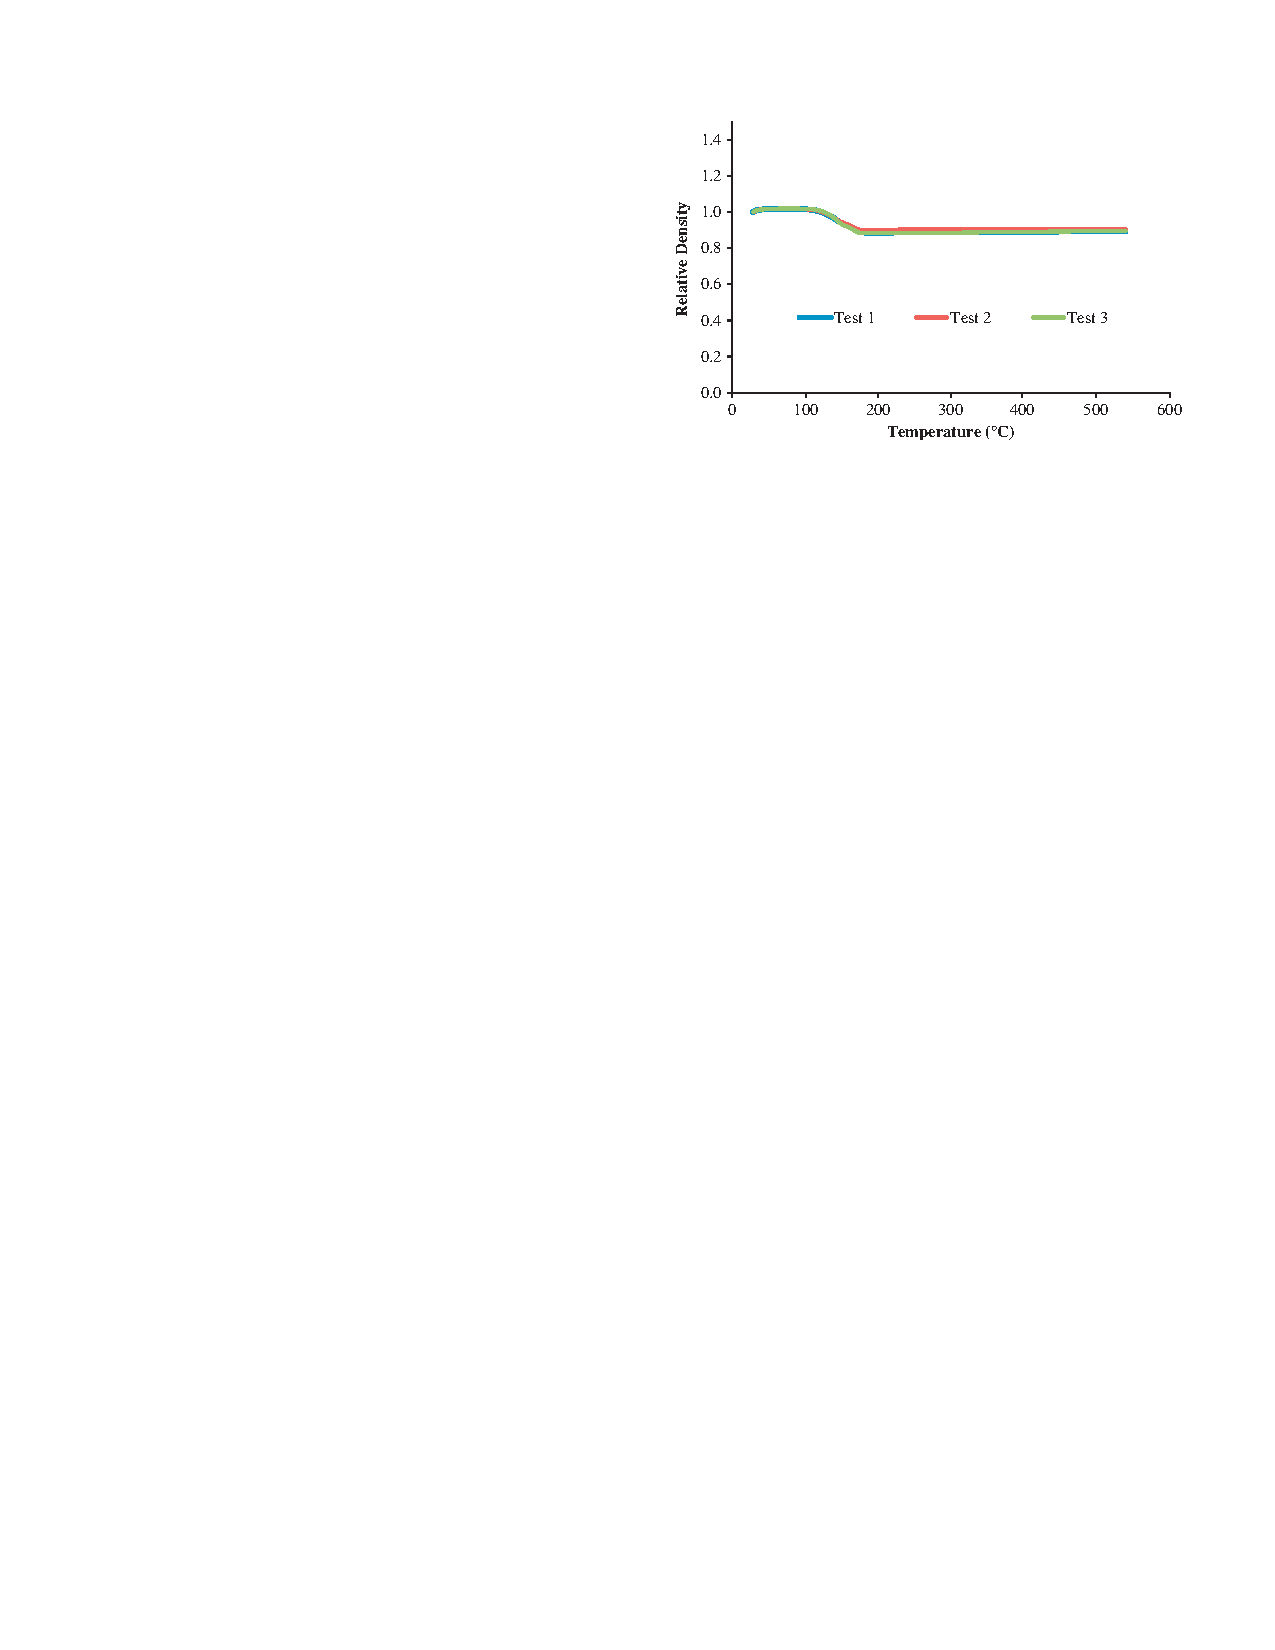
\includegraphics[width=8.5cm,height=6cm]{keerthan_density_measured.pdf} \\
			(b) \\ 
			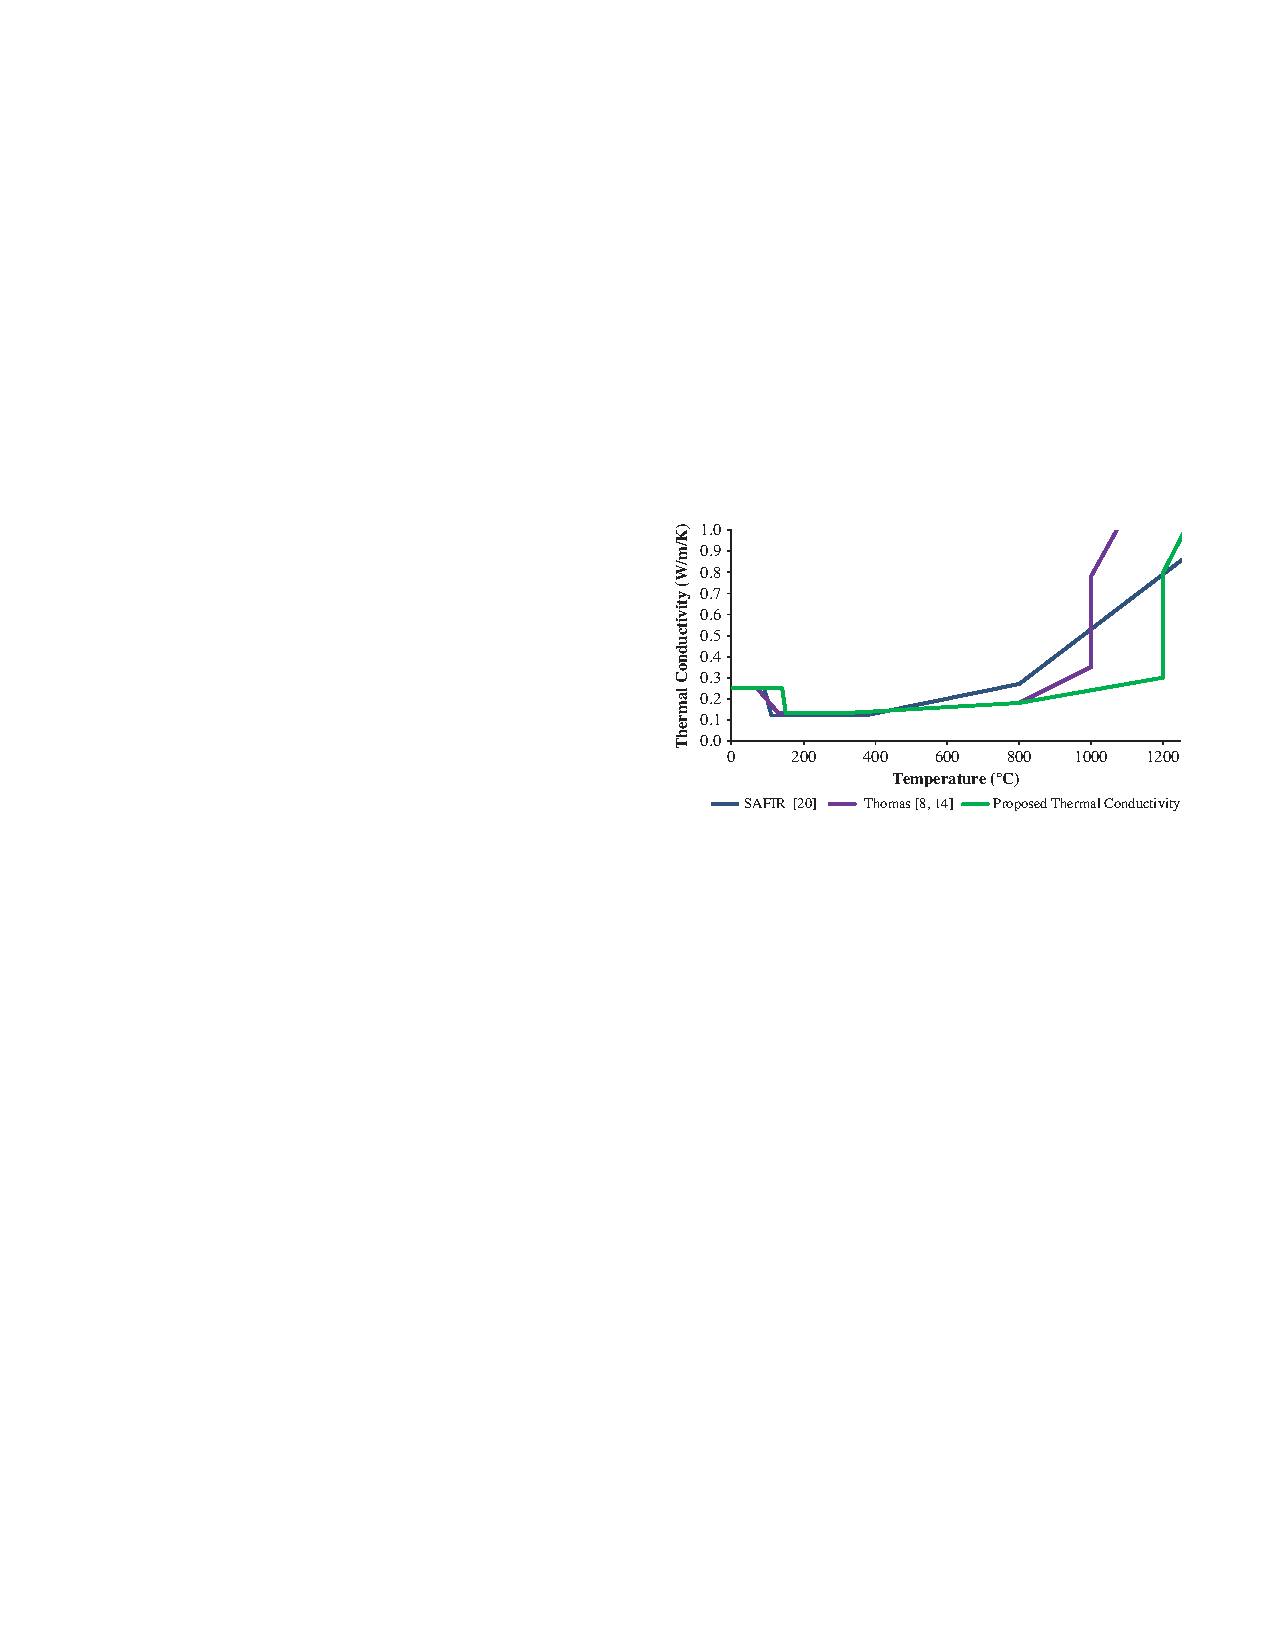
\includegraphics[width=8.5cm,height=5.5cm]{keerthan_conductivity_proposed.pdf} \\
			(c) \\
		\end{tabular} 
		\caption{Proposed thermal properties of plasterboard from \Citet{Keerthan2012a}}
			\label{fig:keerthan_measured}

	\end{figure}

These thermal properties were then used in the FE model developed in SAFIR and the results from the thermal analysis were compared with the results from the small-scale fire tests of plasterboards. It was concluded that, when the default thermal properties in SAFIR were used in the thermal analysis, there was not a good agreement between the FE model and the fire test. However, when the measured thermal properties were used in the thermal analysis, a good agreement was found between the small-scale fire test and FE model. The effect of moisture movement was not considered in the numerical analysis as the effect is not significant in temperatures above 120\degree C.

\Citet{Gunalan2013f} developed structural numerical models and validated them using the experimental results. Initially elastic buckling analysis was conducted using a finite strip analysis software called CUFSM. Various restraint conditions were used to study the elastic buckling behaviour. Then the elastic buckling load was expressed as load factor vs half-wave lengths and the different buckling modes were presented as shown in \Cref{fig:gunalan_buckling}.
\begin{figure}[htbp]
	\centering
		\begin{tabular}{c}
			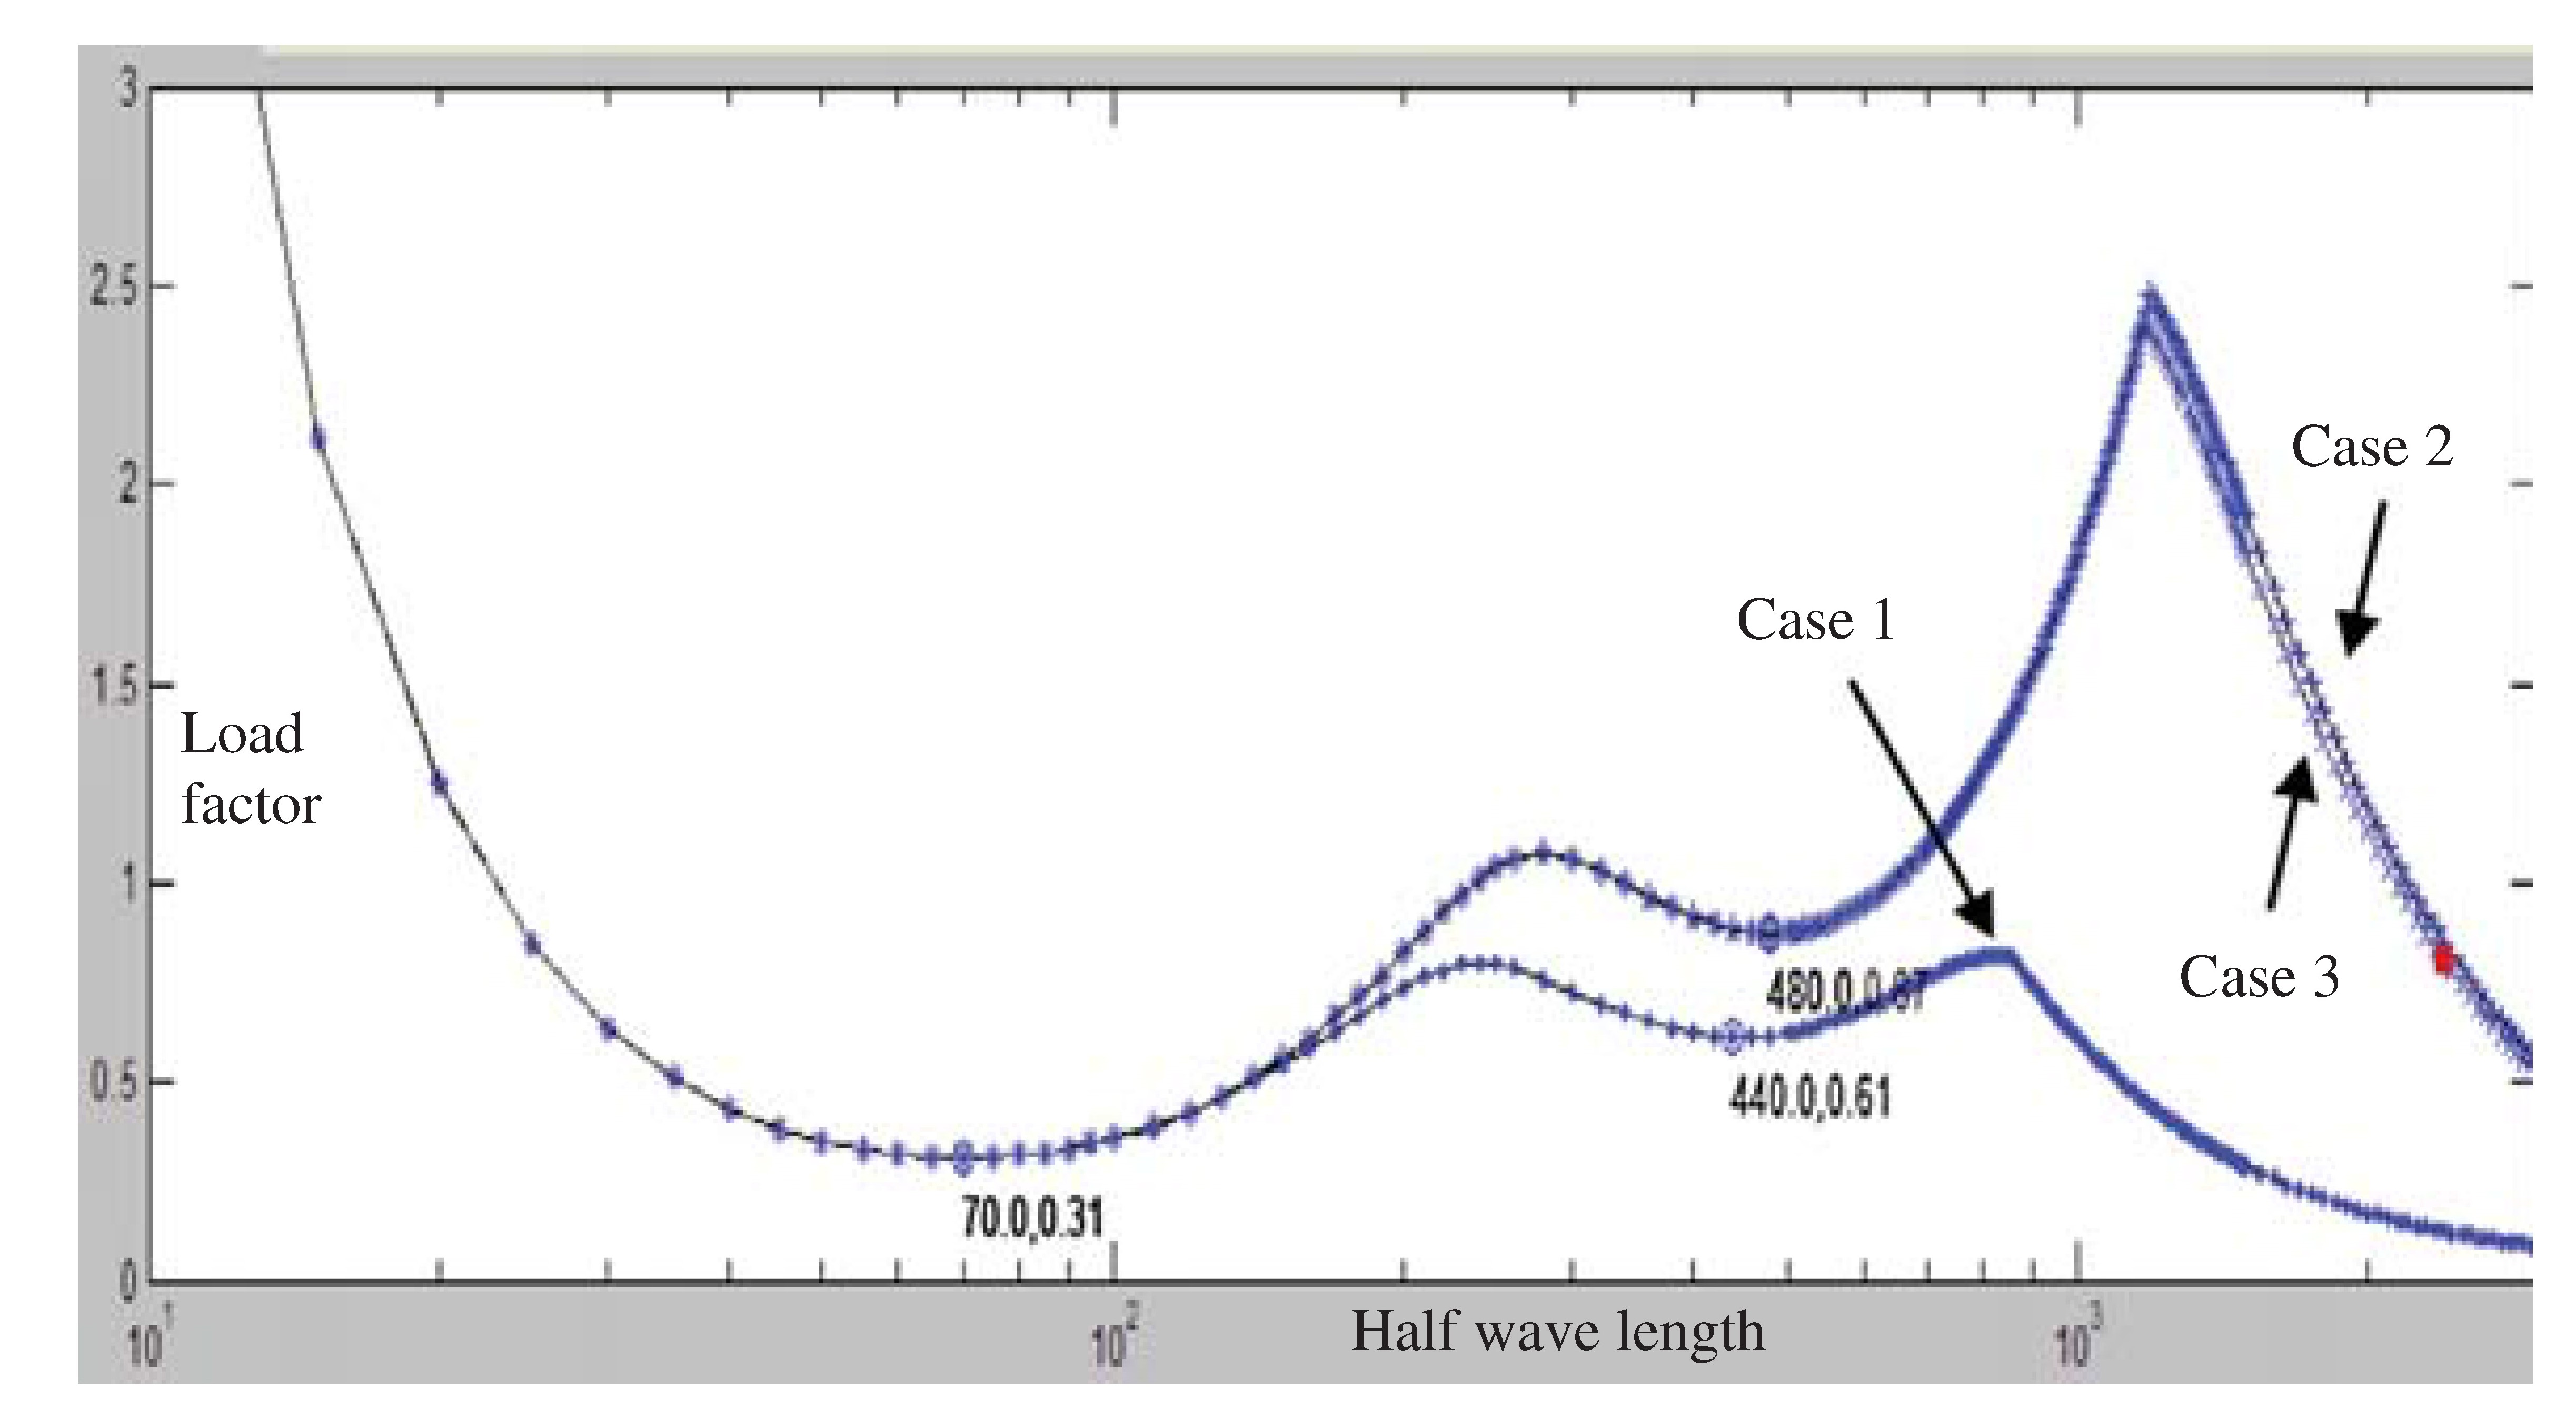
\includegraphics[width=8cm,height=4cm]{gunalan_halfwave} \\ 
			(a)	Load Factor vs Half-Wave Length\\ 
			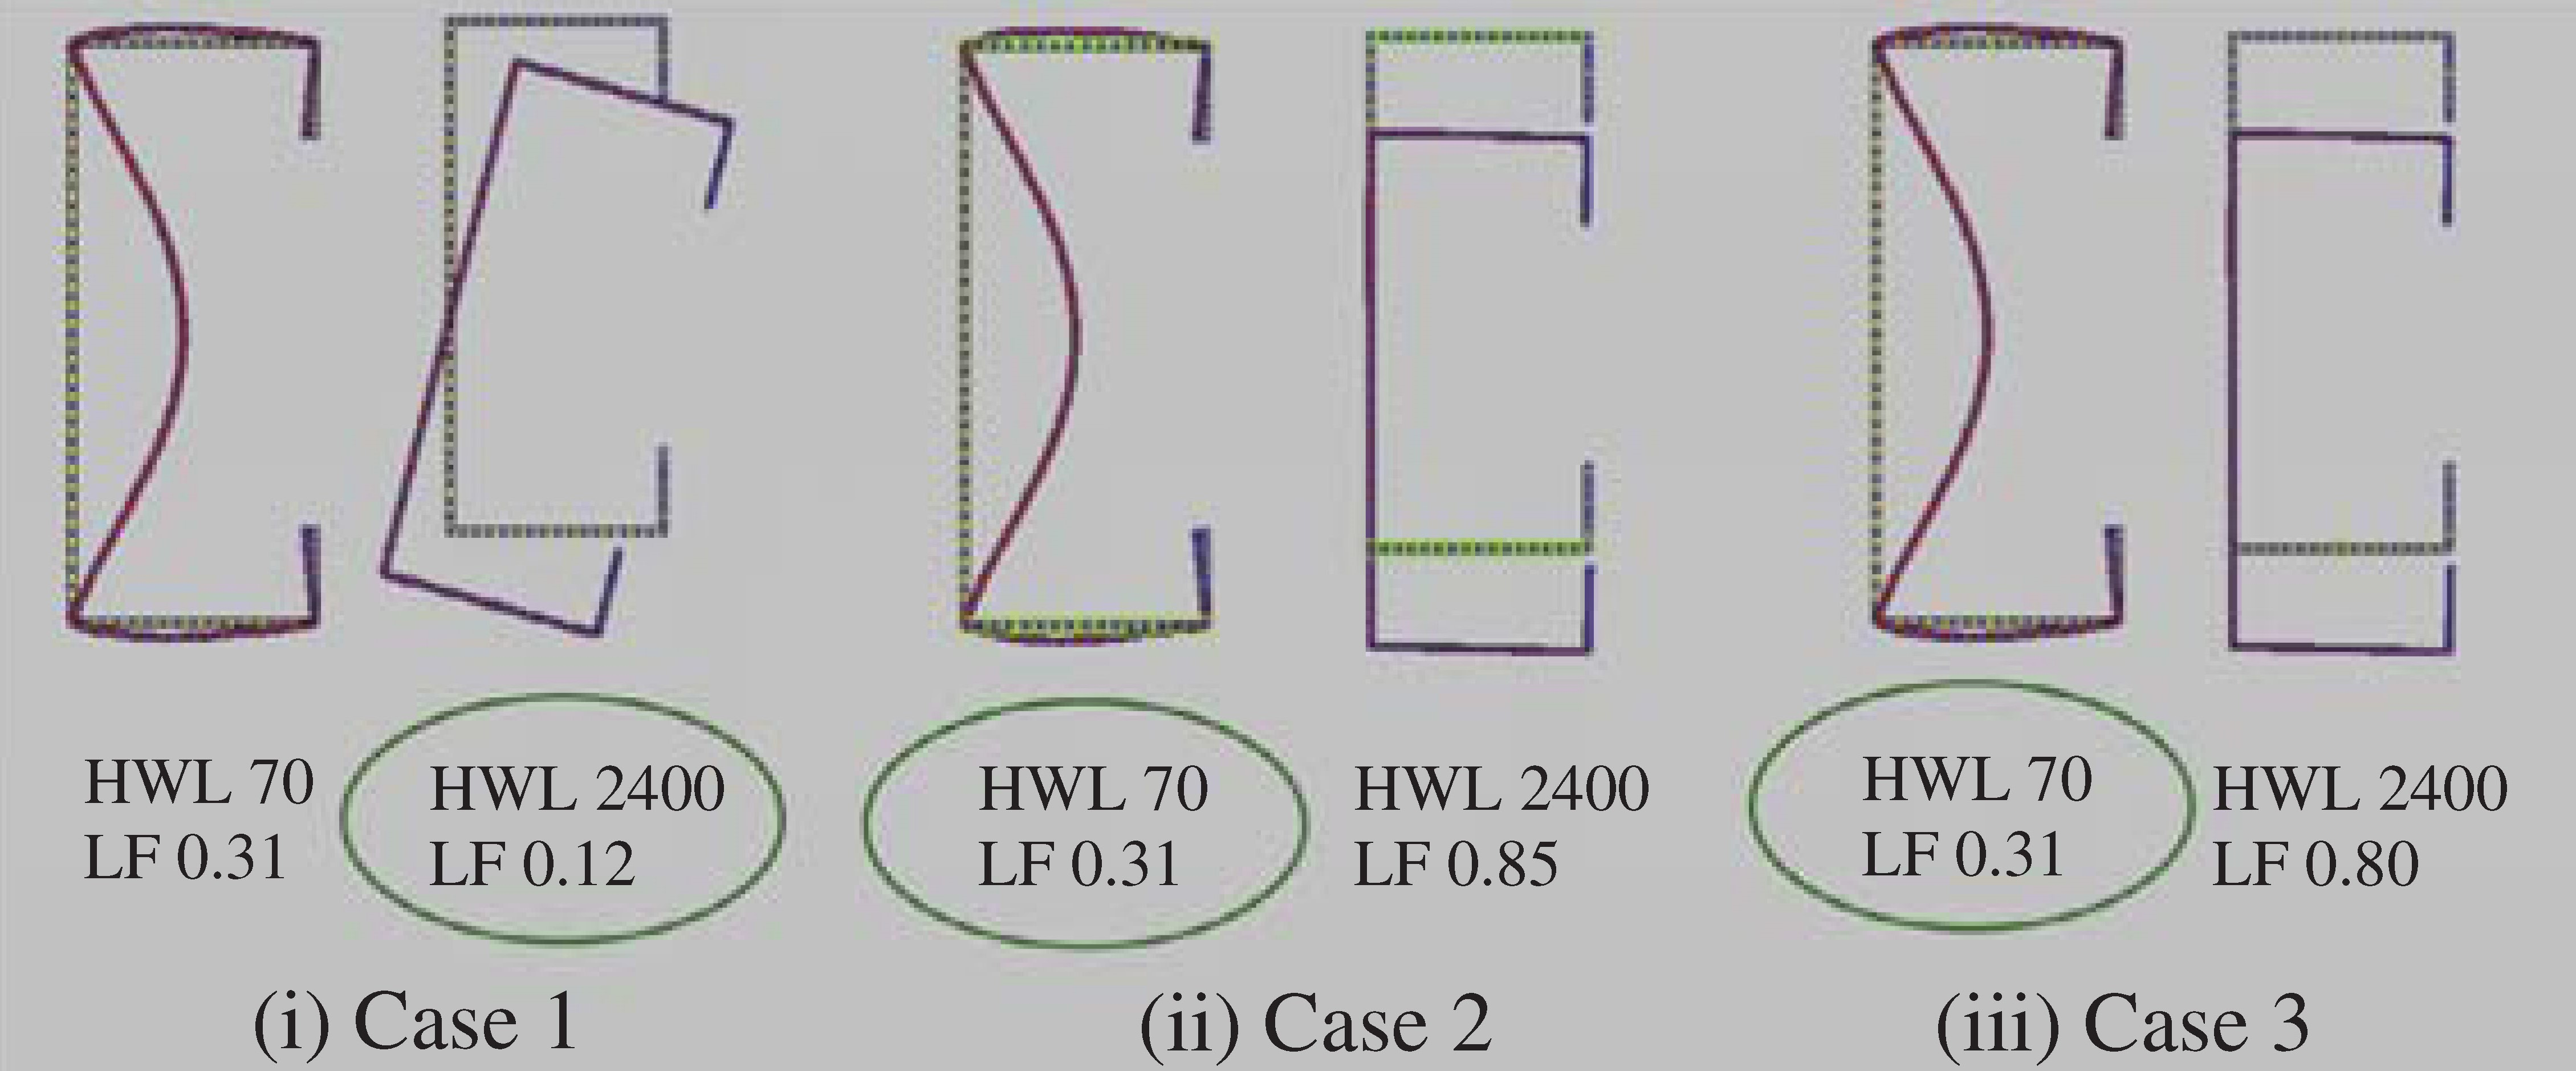
\includegraphics[width=8cm,height=4cm]{gunalan_buckling} \\ 
			(b)	Various Buckling Modes. \\ 
		\end{tabular} 
		\caption{Buckling analysis results from \citet{Gunalan2013f}}
		\label{fig:gunalan_buckling}
\end{figure}

Finite element modelling and analysis were carried out in ABAQUS for the conducted experiments. Mechanical properties such as Young’s modulus were determined by conducting tensile coupon tests. Since ABAQUS accepts true stress and logarithmic plastic strain, the engineering stress and strain from tensile coupon tests were converted to true stress and logarithmic plastic strain using the equations given next.

\begin{equation}
\sigma_{true} = \sigma_{eng}(1+\epsilon_{eng})
\end{equation}

\begin{equation}
\epsilon_{true}^{pl} = \ln(1+\epsilon_{eng})-\dfrac{\sigma_{true}}{E}
\end{equation}

The true stress and logarithmic plastic strain were then fed as input to the structural analysis. Thermal and structural boundary conditions were assumed in accordance with the experiments conducted and non-linear static structural analysis was conducted in ABAQUS. To simplify the thermal boundary conditions, it was assumed that the temperature distribution is linear on the webs from hot flange to cold flange and constant on the flanges. More complex effects such as thermal bowing and deterioration of the mechanical properties at elevated temperatures were studied from the numerical model and validated with the experimental results. New design rules based on AS/NZS 4600 and Eurocode 3 Part 1.3 were proposed by providing allowances for the thermal bowing effects, neutral axis shifts and magnification effects. These proposed design rules were then validated using the results from numerical parametric studies and were found to have good correlation.

\citet{Nassif2014a} proposed a numerical model to predict the transient thermo-mechanical behaviour of LSF walls under fire. Full-scale 3 m $\times$ 3 m wall panels were constructed with single row of studs and gypsum plasterboards were attached on both sides. Sequentially coupled analysis was carried out in ABAQUS and the results were compared with the experimental results. The thermal and mechanical properties for the numerical model were extracted from past literature and Eurocode. The numerical model was developed by considering the transient heat transfer behaviour of the LSF wall during fire. Conduction and convection on the fire exposed and unexposed faces of the wall were considered in the analysis. It was observed from the experiments and numerical models that the plasterboards provide considerable restraints to the steel studs against out of plane deflection. The proposed numerical model predicted the temperature of the steel studs and plasterboard to certain accuracy. However, during the plasterboard fall-off, the temperatures increase rapidly during the experiments and the model could not predict this uncertain behaviour. 

\citet{Chen2014} developed a numerical model to predict the thermal and mechanical response of cold-formed steel (CFS) studs in fire. With the help of measured material properties, a one dimensional thermal response model was formulated to predict the heat transfer mechanism across the width in LSF walls under fire. Gauss-Seidel method was used to solve the governing equations expressed in the form of finite-difference equations. A thermomechanical response model was also developed to predict the axial and lateral deformations in the CFS wall system. Following assumptions were made to simplify the model.
\begin{itemize}
	\item Heat transfer was assumed to happen in the horizontal direction across the width of the wall only. 
	\item Variation in heat transfer due to the steel studs was ignored.
	\item Apparent thermal properties for specific heat were assumed to incorporate the effects of moisture transfer and plasterboard cracking.
	\item Plasterboard cracking was assumed to happen when the temperature increases beyond the threshold limit.
	\item Despite the variation in temperatures along the height of the wall due to the air movement, this effect was neglected in the numerical model.
	\item As the cross-section area of studs is comparatively less than the cavity area, conduction through studs was assumed to be less significant and the corresponding effects were also neglected.
	\item Different failure mode criteria were assumed to predict the failure time for CFS wall assemblies in the thermomechanical model.    
\end{itemize}
Despite the above mentioned simplifications, the numerical model was able to predict the experimental time-temperature and lateral deflection curves with reasonable accuracy. 

\citet{BatistaAbreu2015} proposed advanced numerical modelling of the LSF wall panels. Conventionally, the studs were modelled individually for thermal and structural analysis. However, the plasterboards were also modelled along with the studs and the opening of the joints were assumed, so that, the numerical model simulated the experimental behaviour to greater precision. Sequentially coupled thermal and structural analyses were used in the numerical model developed in ABAQUS. The stiffness of fasteners sheathing system was also investigate numerically as a part of this study. Design equations for normal and fire rated gypsum boards were also proposed. It was concluded that the Finite Strip Method (FSM) and Finite Element Analysis (FEA) are the most efficient methods of structural analysis for cold-formed steel sections.  

\citet{Cheng2015} developed a model to perform buckling analysis of the lipped channel cold-formed steel sections at elevated temperatures. Their investigation was conducted by performing heat transfer analysis initially, followed by pre-buckling and post-buckling analysis. Finite element analysis was used for the heat transfer problem. Bernoulli’s beam theory was used for the pre-buckling analysis by considering the strain effects due to variation in mechanical properties at elevated temperature. Finite strip analysis and classical Fourier solutions were used in the buckling analysis. It was observed that the buckling behaviour of cold-formed steel sections varied under non-uniform temperature exposure when compared with uniform temperature exposure. It was concluded that the higher temperature regions (hot-flange) had lower pre-buckling stresses whereas the lower temperature regions (cold-flange) had higher pre-buckling stresses. Also, the fire design formula for beams under uniform temperature exposure will not be suitable for sections with non-uniform temperature distribution.

The local buckling effects of cold-formed steel compression members were investigated in detail by \citet{Gunalan2015}. Using 91 local buckling tests, experimental results were compared with the numerical predictions from ABAQUS for validation purposes. The cold-formed sections for the local buckling tests were selected using ABAQUS and CUFSM on condition that local buckling occurred at ambient conditions. For elevated temperatures, reduced mechanical properties were used in ABAQUS and CUFSM to find the elastic buckling loads. Shell S4 elements were used in the finite element model. Geometric imperfections proposed by \citet{Schafer2010} for lipped channel sections and \citet{Camotim2006} for plain channel sections were used. Steel grades of G250, G450 and G550 were used in this research. The ambient temperature mechanical properties of G250 and G550 steels were used based on \citet{Ranawaka2009a} while for G450 steel, they were obtained from \citet{Kankanamge2011}. It was concluded that the ambient temperature design rules can be used to predict the buckling behaviour at uniform elevated temperature by considering reduced mechanical properties. The effective area method at ambient temperatures as per Eurocode 3 Part 1.2 resulted in over-conservative results at elevated temperatures. It was also proposed that at elevated temperatures the current design rules can be improvised by incorporating the effects of non-linear stress-strain relationships.

\citet{Kesawan2015a} developed a 2D numerical heat transfer model using SAFIR. The aim of this research was to develop a numerical model for validating the fire tests conducted using HFC steel studs by \citet{Kesawan2015}. A 2D model replicating the fire test was created in SAFIR and the corresponding thermal properties of the materials were keyed in to carry out heat transfer analysis. Heat transfer along the height of the wall was neglected for computational efficiency. GiD, a general purpose pre and post processor software, was used to create models, assign meshes and view the results after analysis. Overall mesh dimension of 8 mm was incorporated into the model based on the research by \citet{Keerthan2012}. Moisture transfer and plasterboard cracking effects were ignored in the thermal analysis considering their insignificant contribution to the FRL. Localised temperature rise in studs due to plasterborard fall-off was also ignored due to the complexity in modelling the same. From the thermal analysis results, it was found that the time-temperature curves of the plasterboards and studs agreed reasonably well with the experimental results in non-cavity insulated HFC walls, while there were minor disagreement with cavity insulated HFC walls. 

A detailed parametric study by considering the variation in stud depth and flange width was also carried out in SAFIR as part of this research. The parametric thermal analysis results shows that the variation in stud time-temperature curves with increase in cavity depth/ stud width did not significantly change. This indicates that, the heat transfer through conduction in stud remains unchanged with increase in cavity depth. However, the time-temperature curves comparison of plasterboards were not presented. It was stated that the same time-temperature profile of studs can be used to determine the FRL irrespective of the cavity depth, which is debatable. The effect of stud thickness was also investigated. Stud thicknesses from 0.6 mm to 3 mm were taken for the parametric study. The thermal analysis results showed that for thicker stud section the hot flange temperatures were lower, while the cold flange temperatures were higher in comparison with the thinner sections. The effect of stud thickness was found to affect the temperature profiles in cavity insulated walls significantly. Increase in stud spacing was also investigated and was found to have no significant effects on the time-temperature curve. The thermal performance of different wall configurations was also investigated. Later, \citet{Kesawan2016} extended the study to develop fire design rules for hollow flange channel sections subjected to non-uniform temperatures under fire. The improved fire design equations were based on AS/NZS 4600 and Eurocode 3 Part 1.3. Direct strength method (DSM) based equation was also proposed and verified based on the experimental and numerical work conducted earlier. The load ratio versus FRL curves derived earlier by \citet{Kesawan2015a} were now obtained using the AS/NZS 4600 and Eurocode 3 design equations. The modified design equations used in this study were based on \citet{Gunalan2013a} along with those from AS/NZS 4600.  

The section moment capacities at stud mid-height and supports were computed by the \Cref{eq:M_mid-height,eq:M_support} shown next.
\begin{equation}\label{eq:M_mid-height}
M_{x,eff} = \dfrac{\bar{f}_{yt}\bar{I}_{eff},t}{y_{max}}
\end{equation}
\begin{equation}\label{eq:M_support}
M_{x,eff} = \dfrac{f_{yt,hf}\bar{I}_{eff},t}{y_{max}}
\end{equation}
The thermal bowing effects were computed based on the modified equation by \citet{Baleshan2016a} as they were found to be less complex and is given in \Cref{eq:bal_e-delta}.
\begin{equation}\label{eq:bal_e-delta}
e\Delta_T = \dfrac{(\alpha_{OHF}OHF-\alpha_{OCF}OCF)L^2}{8d}
\end{equation}
The ratio between end moments $\psi$, was taken as -1 at stud mid-height despite the fact that the value of $\psi$ is greater than -1 and also the actual values. Comparison was made against conventional LCS section with HFC section of similar web depth to understand these effects. The following modifications were made to the design equations. At the stud supports the P-$\Delta$ effects were neglected. Thermal bowing equations from \citet{Baleshan2016a} were used and the actual value of $\psi$ for the bending capacity calculations were computed. Improvements were made to the Eurocode 3 Part 1.3 based equations apart from the AS/NZS 4600 based design equations. Design capacities were also predicted based on the Direct Strength Method (DSM) as well. It was found that the proposed design modifications to the existing equations were able to predict the structural capacities of HFC stud sections in fire to a reasonable accuracy. Comparisons were also made against the FE model predictions from ABAQUS by \citet{Kesawan2016a} to investigate the suitability of these modified design equations. 

Later, \citet{Kesawan2018} reviewed the parameters influencing the fire performance of LSF walls. Important parameters such as plasterboard fall-off, wall configuration, geometric profile of the studs, thermal and mechanical properties of various components at elevated temperatures were discussed in detail based on previously conducted experimental and numerical studies. The effect of plasterboard joints was also discussed in detail. As the fire performance of cavity insulated walls is significantly less in comparison with non-cavity insulated walls, four new LSF wall configurations by externally insulating the walls were proposed in this research. The option of providing plasterboard strips as back blocking to the studs was also proposed to improve the fire performance. However, only limited experimental studies were conducted for the proposed configurations and detailed FE analysis has to be conducted to support the above claims. It was also proposed that the usage of longer fasteners would increase the contact area of screws on plasterboards thereby reducing the plasterboard fall-off during fire. But it is difficult to quantify these effects as substantial experimental and numerical investigations havw not been carried out on these effects. The temperature gradient within the studs was found to have significant influence on the FRL, as the difference in stud hot and cold flanges can result in premature structural failure. Different geometric shaped studs was also proposed and the influence of temperature distribution amongst them was also compared with the help of FE analysis. However, these also need to be validated with the help of experimental studies.

\citet{Ariyanayagam2016} investigated the detrimental effects of plasterboard joints on the fire performance of LSF walls. 150 mm wide plasterboard back blocking was used in the LSF wall panels and standard fire tests were conducted to investigate the detrimental effects of plasterboard joints in fire. Two full scale fire tests at 0.2 load ratio were conducted. The first LSF wall had plasterboard joints between the studs and the second LSF wall had plasterboard joints between the studs with the help of back blocking. The test wall panel was 2.1 m $\times$ 2.4 m with four studs spaced at 600 mm centres. No noggings were used in the LSF wall panel. Fire test results showed that the middle studs (2 \& 3) recorded higher hot flange temperatures in the wall panel, where plasterboard joints were present on the studs when compared to the wall panel with plasterboard joints on back blocking. The failure time of the wall with back blocking plasterboard joint was 74 minutes whereas the conventional specimen lasted only 58 minutes. Numerical investigations were carried out in two steps. Initially, steady state analysis with temperature inputs from the experiments at different time periods were carried out. S4R elements were used for the studs with a mesh size of 4 mm and rigid body with R3D4 elements were used to apply the load to the studs. The studs used in this investigation were made of 1.15 mm G550 steel and were maintained at different temperatures in correspondence with the experiments. The axial compression load was applied and Riks analysis was carried out to achieve the failure of the stud. It was concluded that by providing back blocking to the plasterboard joint in load bearing LSF walls, the FRL of the wall was increased by up to 25\%. However, the plasterboard joints did not have any effect on the non-load bearing LSF walls, which is generally governed by insulation failure.

\citet{Dias2018} developed a thermal FE model in ABAQUS to investigate the thermal behaviour of web-stiffened stud LSF walls in fire. Thermal and structural modelling were conducted for the tested LSF wall configurations using small-scale fire tests. The modelling techniques were adopted from \citet{Rusthi2017}. Web stiffened studs were found to yield better compression capacity under ambient condition in comparison with the conventional lipped channel studs. However, the capacity of the same was not found to provide better results under fire when non-dimensional parameter FRL was considered. The susceptibility of non-load bearing LSF walls failing under structural inadequacy criterion was also discussed based on the conducted FE analysis. However, experimental results were not available to validate this claim. 

\section{Computational Fluid Dynamics (CFD)}

Computational fluid dynamics is a branch of fluid mechanics, in which the numerical problems with respect to fluid flows are solved by numerical analysis and algorithms. Problems related to wind flow and heat transfer are also solved by CFD. The discretization of the problem is undertaken using various methods in CFD such as Finite Element Method, Finite Volume Method, Finite Difference Method, Spectral element method and Boundary element method. Any ideal CFD model will be a dependent of the Navier-Strokes equation.  

To solves a heat transfer problem using a model based on Finite Element Method (FEM), coupled temperature displacement method is used. In this, the conduction, convection and radiation coefficients are used as input to the analysis and the heat transfer problem is solved, whereas in a CFD model these parameters can be input as a 3-D entity to arrive at precise results. ABAQUS CFD / ANSYS Fluent / FDS package is proposed for the numerical analysis of the advanced heat transfer problems to be taken up in this research as part of the numerical validation process.

\citet{Horvat2009} proposed a semi-analytical treatment of wall heat transfer coupled to numerical simulation model of fire. Their objective was to develop a computational technique to predict the heat flow through walls by simulating mass and momentum across the wall when exposed to fire. A numerical heat transfer model was developed in ANSYS CFX. \Cref{fig:horvat_model} shows the 1.2 m long $\times$ 0.8 m wide $\times$ 0.8 m high room considered, which is one third of the ISO room. A 25 mm thick insulation was considered in the walls and ceiling of the model.
\begin{figure}[htbp]
	\centering
		\begin{tabular}{cc}
			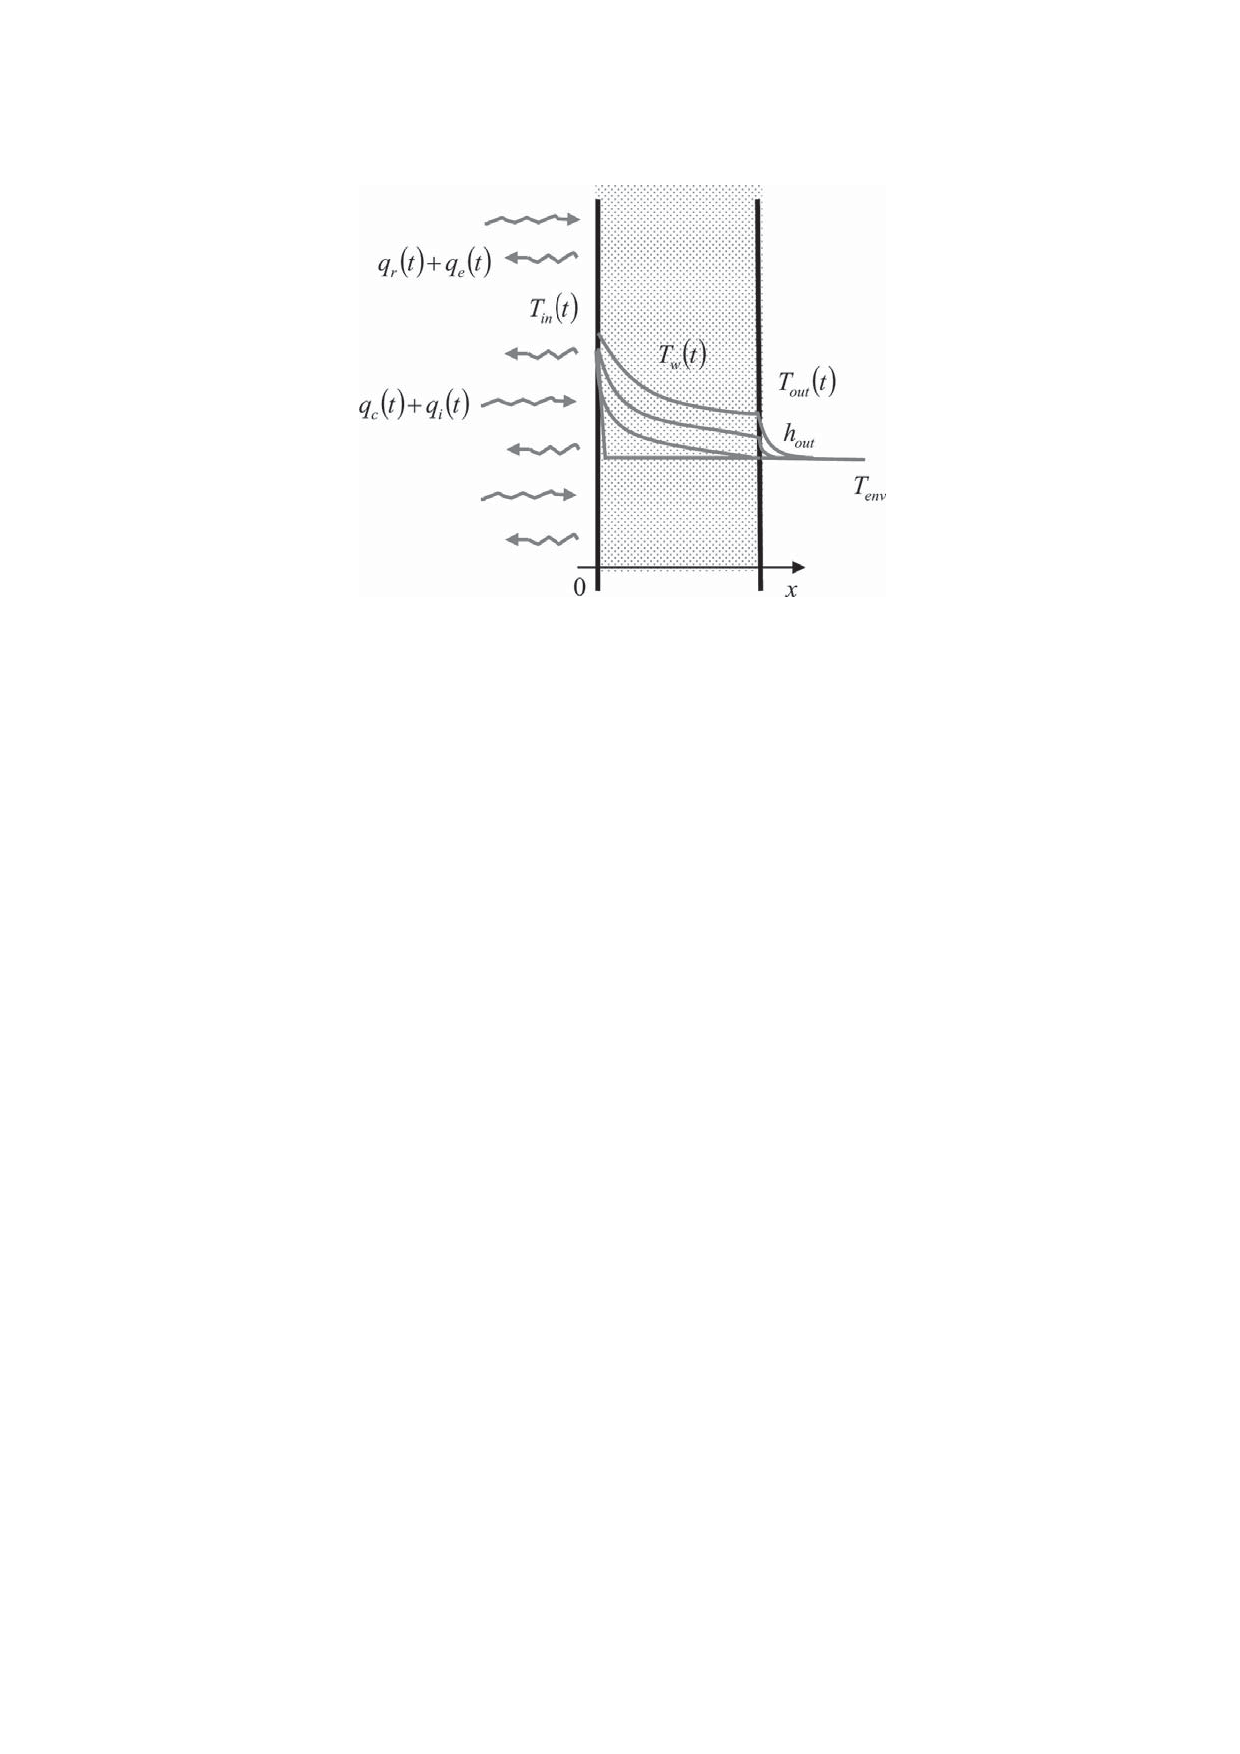
\includegraphics[scale=0.5]{horvat_model} &
			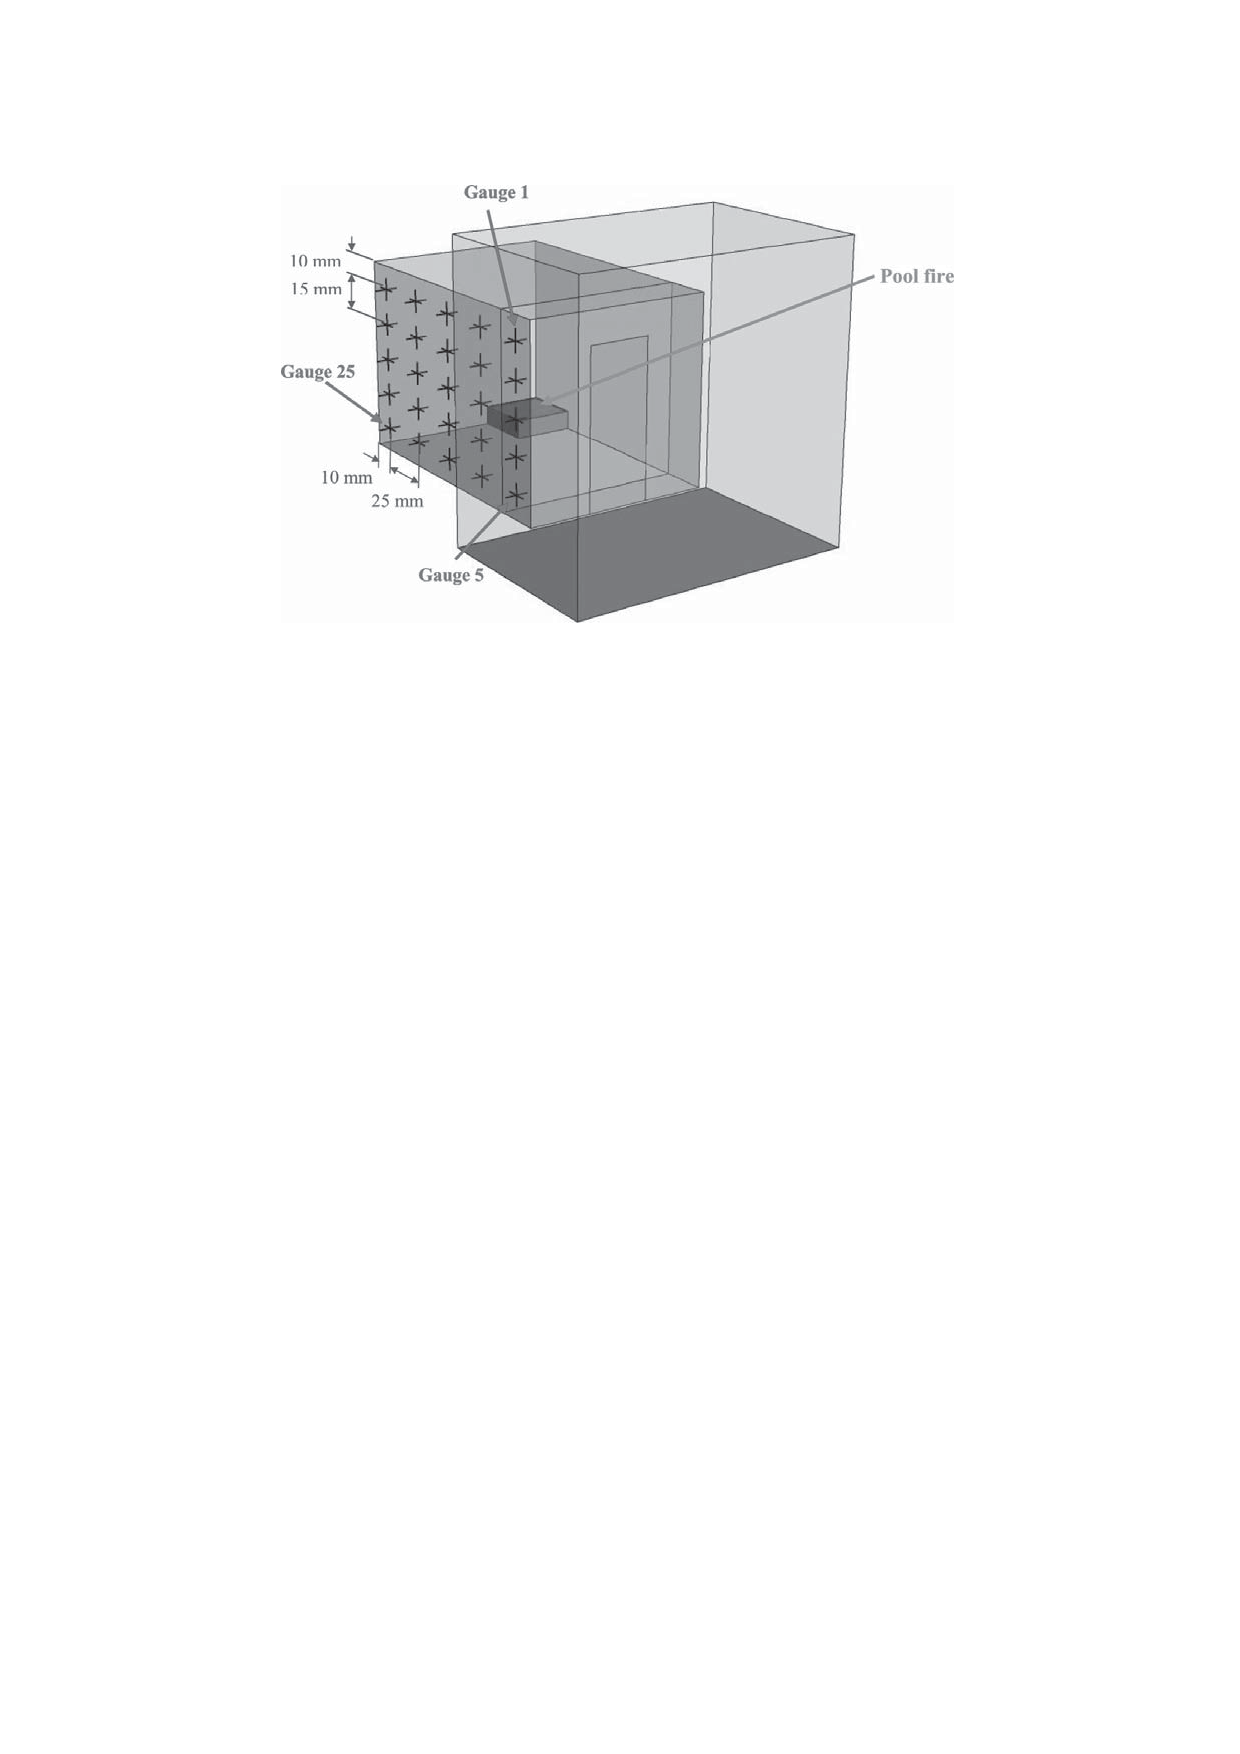
\includegraphics[scale=0.5]{horvat_domain} \\ 
			(a) & (b) \\ 
		\end{tabular} 
		\caption{Modal and domain used by \citet{Horvat2009}}
		\label{fig:horvat_model}
\end{figure}

The fuel boundary was from the back-left corner of the room with sizes of 0.25 m $\times$ 0.25 m with 8 cm elevation. Methanol was used as the fuel source for the inlet boundary condition. This combustion modelling in ANSYS CFX was based on an eddy-dissipation model proposed by \citet{Magnussen1977}. The emissivity of the walls was assumed to be opaque with an emissivity value of 0.9.

The radiation within the cavity is modelled as per discrete transport model. The thermal model of the wall considered in the numerical analysis is shown in \Cref{fig:horvat_model}. The values of thermal heat transfer co-efficient to determine the effect of convection within the cavity were also considered. The convective heat transfer co-efficient $h_w$ varies with time. It was also reported that the heat transfer through the wall takes place by two mechanisms, one through the thermal radiation and the other through the convection of gases. Transient state heat transfer analysis was considered in this study. This developed heat transfer model was validated by comparing its results with experimental results from \citet{Tofilo2005}. The comparison showed good agreement and the benefits of this semi-analytical computational technique. 

The fire resistance of plasterboard entirely depends on the first dehydration point, which takes place at 80\degree C to 250\degree C during fire exposure. Therefore, \citet{Kolaitis2013} developed a solid reaction kinematics dehydration model for gypsum plasterboards exposed to fire in CFD simulations. They addressed the important shortcoming from previous research by \citet{Horvat2009}. The model developed by them included the thermos-physical properties of gypsum plasterboard (density, thermal conductivity and specific heat) and water vapour released from the plasterboard through mass diffusion and convection when exposed to fire. These effects were considered in the model to accurately predict the behaviour of gypsum plasterboards under fire exposure. In this model, the dehydration reactions were not predicted by effective specific heat formulation, whereas two step solid reaction kinematic scheme was used for the predictions. Arrhenius equation was used to estimate the respective reaction rate. Fire Dynamic Simulator (FDS) code was developed based on the above-mentioned criteria and validated with constant thermo-physical property model and an effective specific heat model. The constant thermo-physical model is used as an effective benchmarking model in CFD problems and was used in this research. It was concluded that the proposed CFD model predicted the gypsum plasterboard behaviour with a good agreement level when compared to small-scale fire test results. It was also reported that if the constant thermo-physical properties of the gypsum plasterboard are used, the results showed discrepancies with the experimental results. The quantifying of the water vapour content in the model improves the prediction. 

The influence of wall emissivity and convective heat transfer coefficient within the wall cavity at elevated temperatures was investigated by \citet{Andreozzi2013}. Adiabatic Surface Temperature (AST) model proposed by Wickstrom was investigated with CFD. Conjugate heat transfer analysis is a method that involves the interaction of thermal and structural analysis within the same software. Since this method is computationally very expensive, the AST method is preferred. The AST method used in this study consists of two steps. In the initial step, the thermal analysis was conducted with CFD and later the net heat flux obtained as a result from CFD was transferred to FEM for structural analysis. In this research, conjugate heat transfer analysis and standalone beam analysis were carried out under similar fire exposure and the results were compared. Good agreement was observed between the experimental results and the model when the AST was used as the parameter to transfer CFD results to structural model. The geometry of the model considered was 3 m \(\times\) 3 m with four openings of 200 mm on all sides of the wall.

\citet{Arendt2014} developed a fully transient model of heat transfer in buildings. Transient envelope model and transient CFD model were used to develop this heat transfer model. Reynolds-averaged-Navier-Strokes (RANS) equation was utilized in this research. Higher Reynolds number was used to make the meshes coarser to reduce the computational time during the heat transfer analysis. It was assumed from the CFS solution that there existed a surface-averaged and time-dependent heat transfer coefficient for a given surface. This study was conducted by considering a room with walls possessing thermal capacitance and single ventilation. Developing a transient coarse meshed CFD (RANS) model and transient heat transfer in the building was the principal focus of this research. From the outcomes of this research, it was concluded that the proposed CFD method can be used in reducing the analysis time.

\citet{Lazaro2016} studied the variations in the thermal models used for gypsum plasterboard assemblies in a standard fire test. Numerical analysis results were compared with the experimental results and discrepancies in the current thermal models were reported. Experiments were conducted to determine the thermal and mechanical properties of fire rated gypsum plasterboards. Four full scale fire tests 3 m \(\times\) 3m were conducted with different configurations. Three fire tests consisted of single row of studs, whereas one test consisted of double rows of studs, separated by air gap. All the fire tests were conducted under non-load bearing conditions in accordance with Eurocode EN 1363 and EN 1364. Two layers of fire rated plasterboards were used for three tests and four layers of fire rated plasterboards were used for one test. Sudden increase in temperature was observed on the ambient face of the LSF wall panel after the first plasterboard layer fall-off in the tests with two layers of plasterboards. This was found to be the combined effect of ablation causing convection of hot air within the cavity. Fire Dynamics Simulator (FDS) was used in the numerical study. The model size was 50 mm \(\times\) 50 mm with 5 mm mesh size. Ablation was considered at the third peak reaction corresponding temperature of gypsum in the numerical model. Apparent thermal properties were used in the model to match the numerical results with the experimental results. A new hypothesis was proposed by assuming that the ablation in the plasterboard occurs at about 360\degree C, which was considered as the third endothermic reaction point. It was concluded that the approximation of the thermal properties was held valid for numerical models with two layers of plasterboards. In the case of wall specimen with four layers of plasterboards, the numerical results did not match well with the experimental results. This is because the thermal conductivity between the interface of the plasterboards is difficult to determine causing the discrepancy. Although this research modelled the fire behaviour of LSF walls with CFD only the non-load bearing LSF walls were considered for both experimental and numerical investigations. Also, the temperature gradient along the width of the wall panel was not investigated. The numerical model was validated by comparing the ambient side plasterboard temperatures only.

\citet{Thanasoulas2016} investigated the heat transfer through CFS wall systems through ANSYS CFX software. Structural analysis was conducted using ADINA to determine the structural failure of the CFS walls. Transient heat transfer analysis technique was used for the ANSYS CFX model. Sequentially coupled analysis approach was followed in this study, where the thermal analysis is conducted first and the output is transferred to the structural analysis in the later stages. The models were validated against the experimental results of \citet{Gunalan2013e} and also the FE models developed by \citet{Gunalan2013f}. 2D conduction elements were used in the heat transfer model and the thermo-mechanical properties for the thermal and structural analyses were extracted from \citet{GhaziWakili2007,Kolaitis2013}. A plateau region was observed on the time-temperature curves during the gypsum dehydration process when exposed to the standard ISO fire curve. It was reported that the plateau region happens at 80\degree C, which is debatable. Shell elements were used for structural modelling, wherein the temperature outputs from the thermal analysis were used as input to perform linear and non-linear analyses. Geometric and material non-linearities were included in the structural model. Four full-scale fire tests were considered for the purpose of model validation. It was concluded that, based on the numerical simulations, cavity insulation with mineral wool did not significantly alter the FRL in comparison with non-cavity insulated wall specimen under load bearing conditions, which does not agree with other researchers' findings. The limiting temperature of 350\degree C was found to be conservative for the design of steel studs as the stud load-bearing capacities were satisfactory at the limiting temperature.      

\citet{Malendowski2017} developed a coupling method for CFD-FEM analysis of steel structures exposed to natural fire. Scripts were developed to translate the CFD results into transient boundary condition in FE analysis. The CFD code JASMINE was coupled with an FE code SAFIR. Convective and radiative heat flux are given as input to the FE model. A compartment with dimensions 8 m $\times$ 20 m and 3.2 m high was considered for the computational model as per a full scale fire test conducted by \citet{Pyl2012}. FDS and ABAQUS input files were generated with scripts from Scilab software. UTEMP subroutine was used for defining the boundary conditions in ABAQUS. This UTEMP subroutine was used to create the non-uniform temperature boundary condition in ABAQUS because of heat transfer analysis results from FDS. Real fire curves were used in this study as per \citet{Pyl2012} rather than the standard fire curves used in the furnace fire tests. This is because of the non-uniform radiative heat transfer on the structural elements in the case of a real fire exposure. Pool fire scenario and equally distributed fires were used in the numerical analysis and the results agreed well with experimental results. It was found that the distributed fire scenario is more intense when compared to the local fire by over four times. The deformation plots from structural analysis for both fire scenarios agreed well with the experimental results. 

\citet{Thanasoulas2018} extended the modelling techniques to develop a fully coupled model and to investigate the thermal and structural response of CFS drywall systems. 3-D solid elements were used for modelling the plasterboard, steel studs and insulation to simulate heat transfer through the thickness and also to simulate the structural response in a coupled way. ADINA was used as the software package for the analyses. All the structural elements including the fasteners were modelled in the thermo-mechanical analysis. Appropriate thermal and structural boundary conditions including contact interaction properties were specified along with the elevated temperature material properties. Thermal properties of air was also taken into consideration in the thermo-mechanical analysis. The analysis results showed that the FRL of LSF walls with cavity insulation was higher in comparison with non-cavity insulated LSF walls. This is highly debatable as many other past research studies have shown that the presence of cavity insulation significantly reduces the FRL of LSF walls. 

\section{Literature Review Findings}
The following findings are derived from the conducted literature review.
\begin{itemize}
	\item Fire resistance is considered as an important parameter for walls in LSF constructions. The quantum of research data on the fire resistance of LSF walls is extensive supporting this claim. However, there prevails substantial gaps in this research area, where the fire performance for different fire curves and complex wall configurations has not been investigated in detail. 
	\item Experimental investigations were conducted extensively on simple LSF wall configurations. The tested walls included single row of studs sandwiched between boards of different materials and thickness. This also included the variation in steel stud thickness and grade of steel. But only single row of studs was used in all the experimental investigations. LSF wall configurations with complex stud arrangements were investigated by very few researchers and their fire test data is also not readily available.
	\item Attempts were made to improve the FRL of LSF wall systems by changing various parameters. This includes increasing the number of plasterboard layers on both the fire exposed and unexposed sides, changing the type of insulation used within the cavity and using different geometry of studs. But, attempts were not made to achieve it by the complexity of LSF wall systems by altering their stud arrangements. A research gap is present in relation to the heat transfer mechanism in LSF walls with complex stud arrangements. The presence of more than one row of studs will result in increased cavity depth and change the heat transfer mechanism in comparison with conventional single stud LSF walls.
	\item Many research studies have been conducted on the effect of plasterboard restraints provided to the studs under ambient and fire conditions. However, this effect was investigated only for single stud LSF walls. In the case of complex LSF walls such as double or staggered stud walls, the effective plasterboard restraints varies significantly in certain complex LSF wall configurations. This phenomenon has to be investigated in detail using experimental investigations on the fire performance of complex LSF walls. Also, during a fire test, the LSF wall is subjected to thermal bowing. This effect results in neutral axis shift providing additional bending moments to the LSF walls under axial compression loading. The thermal bowing effect has been investigated in detail for LSF walls with single row of studs only. However, it has not investigated in detail for complex LSF walls.    
	\item Based on the past experimental and numerical research studies, the stud hot flange limiting temperatures have been predicted for different single stud LSF wall configurations such as cavity insulated and non-cavity insulated LSF walls. Through the limiting hot flange temperatures, the FRL of a given wall configuration can be easily derived with reasonable accuracy. But, no such data is available for complex LSF wall configurations. Therefore, it becomes a necessity to investigate the stud hot flange temperatures in complex LSF wall configurations and determine if the existing stud hot flange limiting temperatures are suitable to predict the FRL of complex LSF wall configurations. 
	\item The numerical models developed to predict the heat transfer in LSF walls were through software packages such as SAFIR, ABAQUS, ANSYS, ADINA and FDS. The models were created using 2D and 3D elements and their predictions were compared against experimental results for validation purposes. However, there does not exist a robust numerical model that can predict the heat transfer mechanism in complex LSF wall configurations. Some of the existing heat transfer models included only the radiation mode of heat transfer within the cavity and could still validate the time-temperature curve predictions from the experiments. However, in LSF walls all three modes of heat transfer, conduction, convection and radiation, occur within the cavity. Only numerical models created with CFD software packages could account for these effects. The FE packages such as ANSYS-FLUENT, ADINA and FDS were used by other researchers for developing heat transfer model using CFD techniques, but ANSYS and ADINA are commercial versions and involve a licencing cost while FDS is an open source package. Therefore, FDS is found to be the best option to develop heat transfer models in this research study.
	\item Structural models were also developed by past research studies to predict the structural failure capacities at ambient and elevated temperatures. These models were either sequentially coupled and executed after the thermal analysis or fully coupled and executed alongside the thermal analysis to predict the FRL of LSF walls. However, the fully coupled models were found to be computationally expensive and time consuming. Therefore, sequentially coupled analysis is considered as the preferred method, where the temperature data is extracted from thermal analysis and used in structural analysis.
	\item Numerical models were found to be the most feasible option to predict the FRL of LSF walls. However, the quantum of computational resources and technical skills to conduct these analyses is challenging. Therefore design equations were made available in various standards such as AS/NZS 4600 and Eurocode 3 Part 1.2. Design equations based on the existing standards pertaining to LSF walls were also developed by past research studies. Alternate methods such as DSM and EWM are available to predict the FRL of LSF walls with reasonable accuracy. However, the suitability of these equations for complex LSF walls needs further investigation.
	\item The design equations rely on the hot and cold flange temperatures from either experimental or numerical studies. In single stud LSF walls past research studies assume a constant temperature on the hot and cold flanges while the web temperatures are assumed to be linearly varying. This assumption holds true for LSF wall with single row of studs and the FRL predictions from design equations match reasonably well with the experimental results. However, in complex LSF wall configurations, with more than single row of studs, the applicability of this assumption is questionable. Therefore, extensive experimental and numerical studies are necessary to determine the level of variation in the temperature gradient along the studs. This data can then be used in the design equations to predict the FRL of complex LSF wall configurations.  
\end{itemize}